\documentclass{beamer}

%\usepackage{bookmark}
%\documentclass[handout]{beamer}

\usepackage{bibentry}
\usepackage{femtostslides}
\usepackage[utf8]{inputenc}
\usepackage[english]{babel}
\usepackage{array}
\usepackage[absolute,overlay]{textpos}
\usepackage{xcolor}
\usepackage{amsmath}
\usepackage{multirow}

\usepackage{dirtytalk}
\usepackage{subfigure}

\usepackage{setspace}

\usepackage{etoolbox}

\newtoggle{videoWarning}% enable warning for the videos
\togglefalse{videoWarning}
%\toggletrue{videoWarning}

\usepackage{tikz}
\usetikzlibrary{tikzmark,fit,shapes.geometric,calc}

\newcolumntype{L}[1]{>{\raggedright\let\newline\\\arraybackslash\hspace{0pt}}m{#1}}
\newcolumntype{C}[1]{>{\centering\let\newline\\\arraybackslash\hspace{0pt}}m{#1}}
\newcolumntype{R}[1]{>{\raggedleft\let\newline\\\arraybackslash\hspace{0pt}}m{#1}}

\setbeamercovered{transparent}

\usepackage[absolute,overlay]{textpos}
\usepackage{extrabeamercmds}

\usepackage{adjustbox} % for \adjincludegraphics

\usepackage[boxed]{algorithm2e}
\makeatletter
\newcommand{\removelatexerror}{\let\@latex@error\@gobble}
\makeatother

\makeatletter
\let\oldnl\nl
\newcommand{\nonl}{\renewcommand{\nl}{\let\nl\oldnl}}
\makeatother

\usepackage{amsthm}
\newtheorem{myRule}{Rule}

\definecolor{goodGreen}{RGB}{0,153,0}  % light green
\newcommand{\bad}[1]{\textcolor{red}{#1}}
\newcommand{\good}[1]{\textcolor{goodGreen}{#1}}

%%% Alg
\let\argmax\relax
\DeclareMathOperator*{\argmax}{argmax}
\DeclareMathOperator*{\argmin}{argmin}

\newcommand{\MyAlgoCapSpace}{0.5em}
\newcommand{\MyAlgoDecSpace}{0em}
\newcommand{\MyAlgoIndentSpace}{0em}
\newcommand{\mySpaceInterval}{0em}
\newcommand{\decMarginLength}{1.3em}

\SetAlFnt{\footnotesize}
\SetAlCapSkip{1em}

\SetKwData{Left}{left}
\SetKwData{This}{this}
\SetKwData{Up}{up}
\SetKwFunction{Union}{Union}
\SetKwFunction{FindCompress}{FindCompress}
\SetKwFor{ForEach}{for each}{do}{end}
\SetKwProg{Fn}{Function}{:}{end}		

\SetKwInOut{Settings}{Settings}
\SetKwInOut{Input}{Input}
\SetKwInOut{Output}{Output}  
\SetKwInOut{Variants}{Variants}
\SetKwInOut{Primitives}{Primitive(s)}
\SetKwInOut{Variables}{Local Variables}  

\newcommand{\myAlgParam}[2]{
	\begin{figure}[#1]
		\IncMargin{\decMarginLength}
		\removelatexerror	
		\begin{algorithm}[H]
			#2
		\end{algorithm}
		\DecMargin{\decMarginLength}
	\end{figure}
}

\newcommand{\myAlg}[1]{
	\myAlgParam{!h}{#1}
}

\makeatletter
\def\beamer@startmycovered{%
	\def\opaqueness<##1>##2{%
		\only<##1>{%
			\beamer@actions{%
				\expandafter\xdef\csname beamer@oldcolorhook%
				\the\beamer@coveringdepth\endcsname{\beamer@colorhook}%
				\expandafter\xdef\csname beamer@oldpgfextension%
				\the\beamer@coveringdepth\endcsname{\beamer@pgfextension}%
				{\globalcolorstrue\colorlet{beamer@freeze\the\beamer@coveringdepth}{bg}}%
				\xdef\beamer@colorhook{!##2!beamer@freeze%
					\the\beamer@coveringdepth\beamer@colorhook}%
				\gdef\beamer@pgfextension{!##2opaque}%
				\color{.}%
			}%
			{%
				\xdef\beamer@colorhook{\csname beamer@oldcolorhook%
					\the\beamer@coveringdepth\endcsname}%
				\xdef\beamer@pgfextension{\csname beamer@oldpgfextension%
					\the\beamer@coveringdepth\endcsname}%
				\color{.}%
	}}}%
	\ifnum\beamer@slideinframe<\beamer@minimum%ok, at beginning
	{%
		\beamer@saveanother%
		\advance\beamer@minimum by-\beamer@slideinframe%
		\beamer@slideinframe=\beamer@minimum%
		\beamer@uncoverbeforeactions%
		\beamer@restoreanother%
	}%
	\else%
	{%
		\beamer@saveanother%
		\advance\beamer@slideinframe by-\beamer@minimum%
		\beamer@uncoverafteractions%
		\beamer@restoreanother%
	}%
	\fi%
	\beamer@do%
	%  }%
}

\long\def\beamer@makemycovered#1{\beamer@startmycovered#1\beamer@endcovered}
\def\mycover{%
	\alt{\beamer@makemycovered}{\beamer@fakeinvisible}}
\def\c@slideinframe{\beamer@slideinframe}
\makeatother

\newcommand{\remarkColor}{femtostdarkblue}

\newcommand{\remark}[1]{
	\begin{center}
	 \textcolor{\remarkColor}{$\implies$ #1}
	\end{center}
}
	
\title[Thesis Defense]{Distributed Algorithms for Large-scale Robotic Ensembles: Centrality, Synchronization and Self-reconfiguration}

\subtitle{Thesis Defense}

\author[A. Naz]{André Naz\inst{1}\\Thesis Defense\\\insertdate\\~\\\underline{Supervisors:} Julien Bourgeois, Seth C. Goldstein and Benoît Piranda} 
%\\~\\\underline{Jury members:} Kay Römer, Roger Wattenhofer, Nikolaus Correll}
\institute[{UBFC-UFC-FEMTO-ST}]{\inst{1} Univ. Bourgogne Franche-Comté, University of Franche-Comté\\FEMTO-ST Institute, CNRS}

\date{December, 4 2017}

\setLogoFirstPageCmd{\vspace{-12pt}\hspace*{-3.5cm}
\includegraphics[scale=0.5]{fig/logos/logo-first-page.pdf}\vspace{-12pt}}

% Disable all logos!
\setLogoCmd{}%
\includegraphics[scale=0.5]{fig/logos/logo.pdf}\kern 5pt\vspace{-10pt}}

\newcommand{\noLogo}[1]{{\setLogoCmd{}#1}}

\begin{document}

\begin{frame}

\iftoggle{videoWarning}{
   \vspace{-3em}
}{}

   \titlepage

\iftoggle{videoWarning}{  
   \begin{textblock*}{0.97\paperwidth}(0.03\paperwidth,0.675\paperheight)
   	\begin{center}	
   		\begin{columns}[c]
   			\begin{column}{0.02\textwidth}
   				\centering
   				%\vspace*{-1em}
   				\warning{}
   			\end{column}
   			\begin{column}{.98\textwidth}
   				\small
   				\centering			
   				\textcolor{\remarkColor}{The original presentation contains videos that are not embedded in this PDF.\\Please visit~\url{https://github.com/nazandre/phdthesis-defense}\\to visualize the videos.}
   			\end{column}
   		\end{columns}
   	\end{center}
   \end{textblock*}
}{}
   
  \begin{textblock*}{0.25\paperwidth}(0.725\paperwidth,0.835\paperheight)
  \begin{center}
  \tiny Funded by the ANR/RGC (contracts ANR-12-IS02-0004-01 and 3-ZG1F)
  \end{center}
  \end{textblock*}
\end{frame}

\begin{frame}
  \frametitle{\ensiflanguage{french}{Sommaire}{Outline}}
  \tableofcontents[subsectionstyle=hide,subsubsectionstyle=hide]
\end{frame}

{ 
\AtBeginSection[]{}
\section{Introduction}


\newcommand{\contextSubSectionOneTitle}{A Broad Context:\\From the IoT to Large-scale Robotic Ensembles}

%A Broad Context: From the IoT to
\subsection{Large-scale Robotic Ensembles}

\newcommand{\iotversion}[1]{fig/Iot/#1}

\newcommand{\iotslide}[2]{
\noLogo{
\begin{frame} \frametitle{\contextSubSectionOneTitle{}}
	
	\begin{center}
		\begin{columns}[c]
			\begin{column}{.33\textwidth}
				\vspace{1cm}
				\begin{center}
					\includegraphics[width=\linewidth]{\iotversion{#1}}
				\end{center}
			\end{column}
			\begin{column}{.66\textwidth}
					#2
			\end{column}
		\end{columns}
	\end{center}
\end{frame}
}
}

\noLogo{
	\begin{frame} \frametitle{Large-scale Robotic Ensembles}
	
	\vspace{-0.5cm}
	\begin{center}
		\begin{columns}[c]
			\begin{column}{.25\textwidth}
				\centering
				\includegraphics[width=\linewidth]{\iotversion{iot-oval-lre}}
			\end{column}
			\begin{column}{.75\textwidth}
				
					{
					\setbeamercovered{invisible}
					%Large-scale robotic ensembles:
					\begin{itemize}
						\item Modular robotics, swarm robotics, distributed MEMS, robotic materials
						\item Macro-scale: reconfigurable IoRT objects
						\item Micro-scale: self-organized ensembles 
						\begin{itemize}
							\item up to $10^6$ units
							\item small and resource-constrained (energy, memory, computation) units 
						\end{itemize}
						\item Advantages: versatility, robustness, cheaper
					\end{itemize}
					}	
			\end{column}
		\end{columns}
	
		\begin{columns}[c]
			\begin{column}{.5\textwidth}
				\centering
				\href{run:videos/3-smartblocks.avi?autostart&loop}{\adjincludegraphics[width=0.9\linewidth,valign=c]{videos/3-smartblocks.jpg}}\\
				Conveying Surface\\Smart Blocks project (FEMTO-ST)
			\end{column}
			\begin{column}{.5\textwidth}
				\centering
				\href{run:videos/3-claytronics.mp4?autostart&loop}{\adjincludegraphics[width=0.9\linewidth,valign=c]{videos/3-claytronics.jpg}}\\
				Programmable Matter\\Claytronics project (CMU)
			\end{column}
		\end{columns}
		
	\end{center}
	
\end{frame}
}


\subsection{An Inter-Disciplinary Domain}

%A Caricatural Vision
\definecolor{thisThesisColor}{RGB}{255,204,0} 
\begin{frame} \frametitle{An Inter-Disciplinary Domain}

\begin{center}
\begin{columns}[c]
	\begin{column}{.6\textwidth}
		\centering
		\only<1>{
		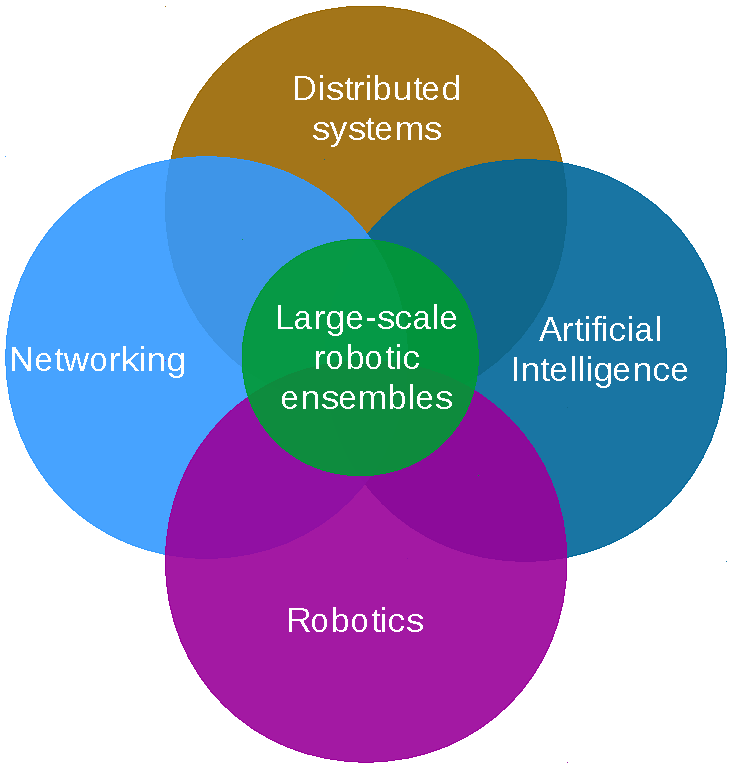
\includegraphics[width=\textwidth]{fig/domains/domains-not-positioned}
		}
		\only<2>{
		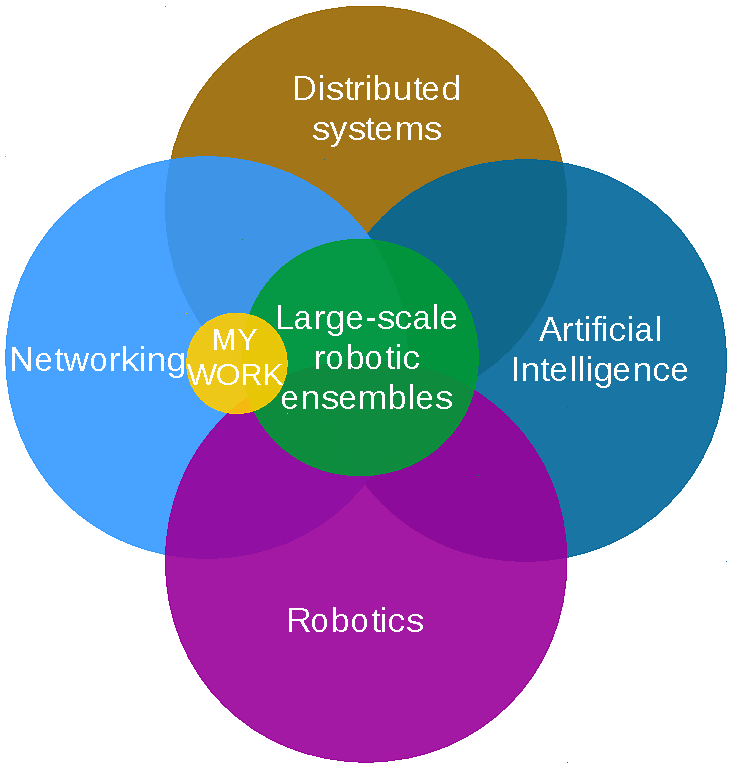
\includegraphics[width=\textwidth]{fig/domains/domains}
		}
	\end{column}
	\begin{column}{.4\textwidth}		
		Challenges:
		\begin{itemize}
			\item Hardware: Fabrication
			\item \tikzmark{start}Algorithmic: Distributed \tikzmark{end} coordination
		\end{itemize}
	\end{column}
\end{columns}
\end{center}

\begin{tikzpicture}[remember picture,overlay]
\draw<2>[draw, line width=2pt,thisThesisColor,label={[xshift=1.0cm, yshift=-0.15cm,align=center]\textcolor{thisThesisColor}{My work}}] (9.92,3.5) ellipse (2.5 and 0.6);
\node<2> at ($(9.92,2.6)$) {\textcolor{thisThesisColor}{my work}};
%
%\node<2>[draw,line width=2pt,cyan,circle,fit={(pic cs:start) (pic cs:end)}] {};
\end{tikzpicture}

\end{frame}

\subsection{Problem Statement}

\begin{frame} \frametitle{Problem Statement}

{
\setbeamercovered{invisible}
\begin{itemize}
\item<1-> Coordination of large-scale ensembles of resource-constrained robots\\
\textcolor{femtostdarkblue}{$\implies$ New algorithmic challenges}\\
\textcolor{femtostdarkblue}{$\implies$ My postulate: we need to identify and design high-level primitives to help the coordination of these ensembles}
\item<2-> Application scenario*:

  \begin{columns}[c]
	\begin{column}{.45\textwidth}
		\centering
		\only<2-> {
		\adjincludegraphics[width=\linewidth]{fig/scenario/base-application}
		}
	\end{column}
	\begin{column}{.1\textwidth}
		\centering
		\only<3-> {
			\adjincludegraphics[width=0.8\linewidth]{femtostslides-files/fig/blue-bits-icons-256x256/1_036}
		}
	\end{column}  
	\begin{column}{.45\textwidth}
		\centering
		\only<3-> {
			\href{run:videos/5-scenario.avi?autostart&loop}{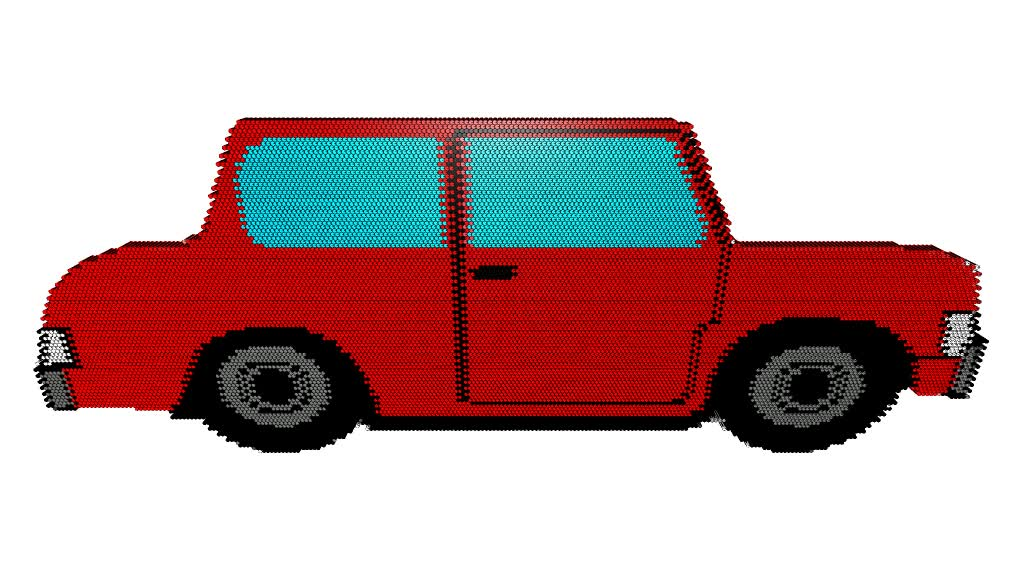
\includegraphics[width=\linewidth]{videos/5-scenario.jpg}}
		}
	\end{column} 
\end{columns}
\vspace{-0.5cm}
\item<4-> Research problems (proposed high-level primitives):
		\begin{enumerate}
			\item Shape construction
			\item Time synchronization
			\item Centrality-based leader election
		\end{enumerate}
\end{itemize}
}
\only<2-> {
	\begin{textblock*}{0.96\paperwidth}(0.02\paperwidth,0.88\paperheight)
		\tiny
		%\footnotesize 
	{
		\setstretch{0}
		\begin{center}			
			*Image based on modified versions of images released in the public domain under the Creative Commons CC0 license which were downloaded from \href{https://pixabay.com/fr/loupe-grossissant-transparent-303408/}{Pixabay} and  \href{http://fotomelia.com/?download=clipart-illustration-voiture-rouge-images-photos-gratuites}{Fotomelia}.
		\end{center}
	}
	\end{textblock*}
}
\end{frame}
}

\section{Research Environment: Hardware and Simulation Tools}

%\subsectionOutlineFrame

\noLogo{
\begin{frame} \frametitle{The Blinky Blocks}

\begin{itemize}
	\item Several generations:
		\begin{itemize}
			\item Originally developed at Carnegie Mellon University~\cite{Kirby-chi11}
			\item Last generations fabricated by FEMTO-ST
		\end{itemize}
	\item Hardware features
	\begin{itemize}
		\item micro-controller: ATMEL ATxmega256A3-AU 8/16-bits 32MHz
		\item memory: 256KB ROM and 16KB RAM
		\item Network: 6 serial interfaces configured at 38.4 kbit/s
		\item RGB leds
		\item Local Clock: Real-Time Counter driven by a RC oscillator
		\begin{itemize}
			\item 1\% accuracy and 1ms resolution
		\end{itemize}
	\end{itemize}
\end{itemize} 

\begin{center}
	\begin{columns}[c]
		\begin{column}{.50\textwidth}
			\centering
			\adjincludegraphics[width=.8\linewidth,valign=t]{fig/environment/bb-details.png}\\
		\end{column}
		\begin{column}{.50\textwidth}
			\centering
			\adjincludegraphics[width=.8\linewidth,valign=t]{fig/environment/bb-rainbow.png}\\
		\end{column}
	\end{columns}
\end{center}
\end{frame}
}


\noLogo{
	\begin{frame} \frametitle{The 2D Catoms}
	
	Partially validated	2D Catom hardware prototype \cite{karagozler-iros09}
	
	\begin{columns}[b]
		\begin{column}{.55\textwidth}
			\centering
			\href{run:videos/8-2dcatom.avi?autostart&loop}{\adjincludegraphics[width=0.8\linewidth,valign=c]{videos/8-2dcatom.jpg}}\\
			Hardware prototype
		\end{column}
		\begin{column}{.4\textwidth}
			\begin{center}
				\adjincludegraphics[width=0.8\linewidth,valign=c]{fig/environment/catom_actuation.png}\\
				Actuation scheme
			\end{center}
		\end{column}
	\end{columns}	 
	
	Partially validated: 
	\begin{itemize}
		\item Only motion on the ground
		\item No communication, nor module arrangement, nor color for now
	\end{itemize}
\end{frame}
}

\noLogo{
\begin{frame} \frametitle{VisibleSim}
	
	Simulator of modular robotic ensembles~\cite{dhoutaut2013efficient}
	
	\begin{center}
		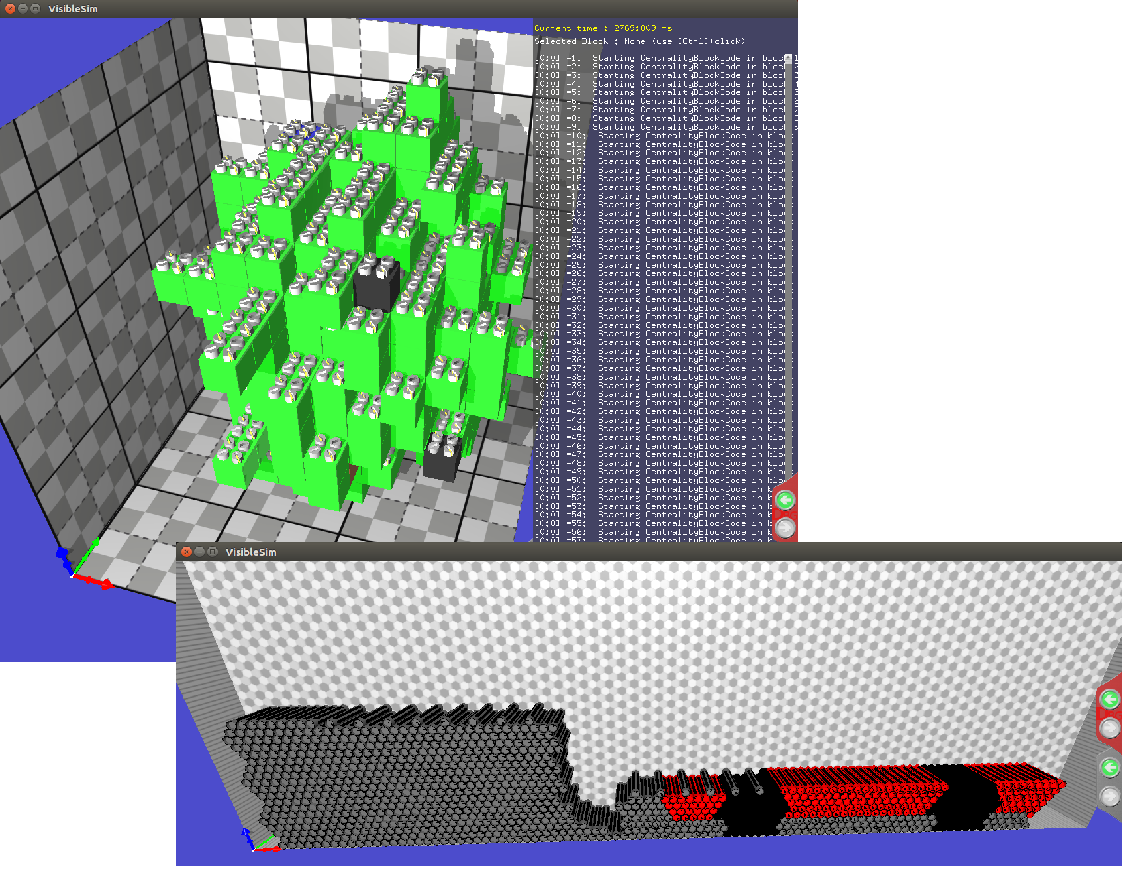
\includegraphics[width=.8\linewidth]{fig/environment/vs}
	\end{center}

\end{frame}
}

\section{Centrality-based Leader Election}

\subsection{Problem and Motivations}

\noLogo{
\begin{frame} \frametitle{Problem and Motivations}

{
\setbeamercovered{invisible}
\begin{itemize}

\item<1-> Network graph G(V,E): V = modules, E = connections\\
\begin{itemize}
	\item<1-> Neighbor-to-Neighbor communications, unique node identifiers
	\item<1-> $d(v_i, v_j)$ = hop distance between modules $v_i$ and $v_j$
\end{itemize}

\item<2-> Problem: efficient election of an approximate central node

\item<3-> Central nodes?
\begin{itemize}

\item<4-> Center: minimizes the maximum distance to all the others\\
\hspace{2cm}$Center = \argmin\limits_{v_i \in V} ecc (v_i) = \argmin\limits_{v_i \in V} \max\limits_{v_j \in V} d(v_i,v_j)$

\item<5-> Centroid: minimizes the average distance to all the others\\
\hspace{2cm}$Centroid = \argmin\limits_{v_i \in V} \frac{1}{|V|} \sum\limits_{v_j \in V} d(v_i,v_j)$ 

%\item Betweenness center: nodes on most shortest-paths
\end{itemize}

\item<6-> Challenge: requires a distributed all-pair shortest path computation
	\begin{itemize}
		\item Large time, message and/or storage costs.	
	\end{itemize}

\item<7-> Motivation: ideal nodes for communications with all the others
	\begin{itemize}
		\item Example: service providers
			\begin{itemize}
				\item Time synchronization: the precision decreases with the hop distance to the time master
			\end{itemize}
	\end{itemize}
\end{itemize}
}

\only<1-3>{
	\begin{textblock*}{\paperwidth}(-0.5cm,0.57\paperheight)
		\begin{figure}
	  		\centering
	  		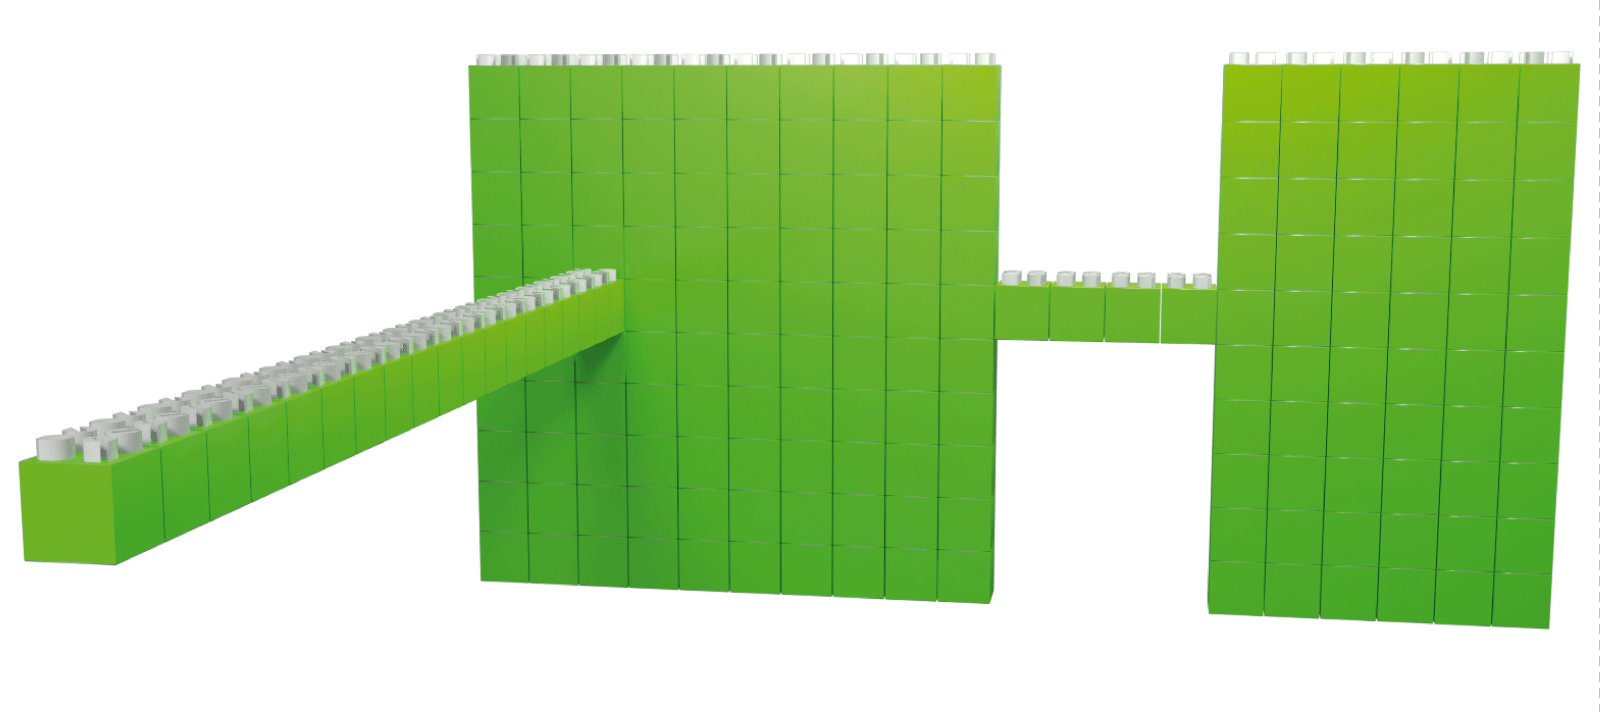
\includegraphics[height=0.35\paperheight]{fig/centrality/centers/initial}
	  	\end{figure}
	\end{textblock*}
}

\only<4>{
	\begin{textblock*}{\paperwidth}(-0.5cm,0.57\paperheight)
		\begin{figure}
			\centering
			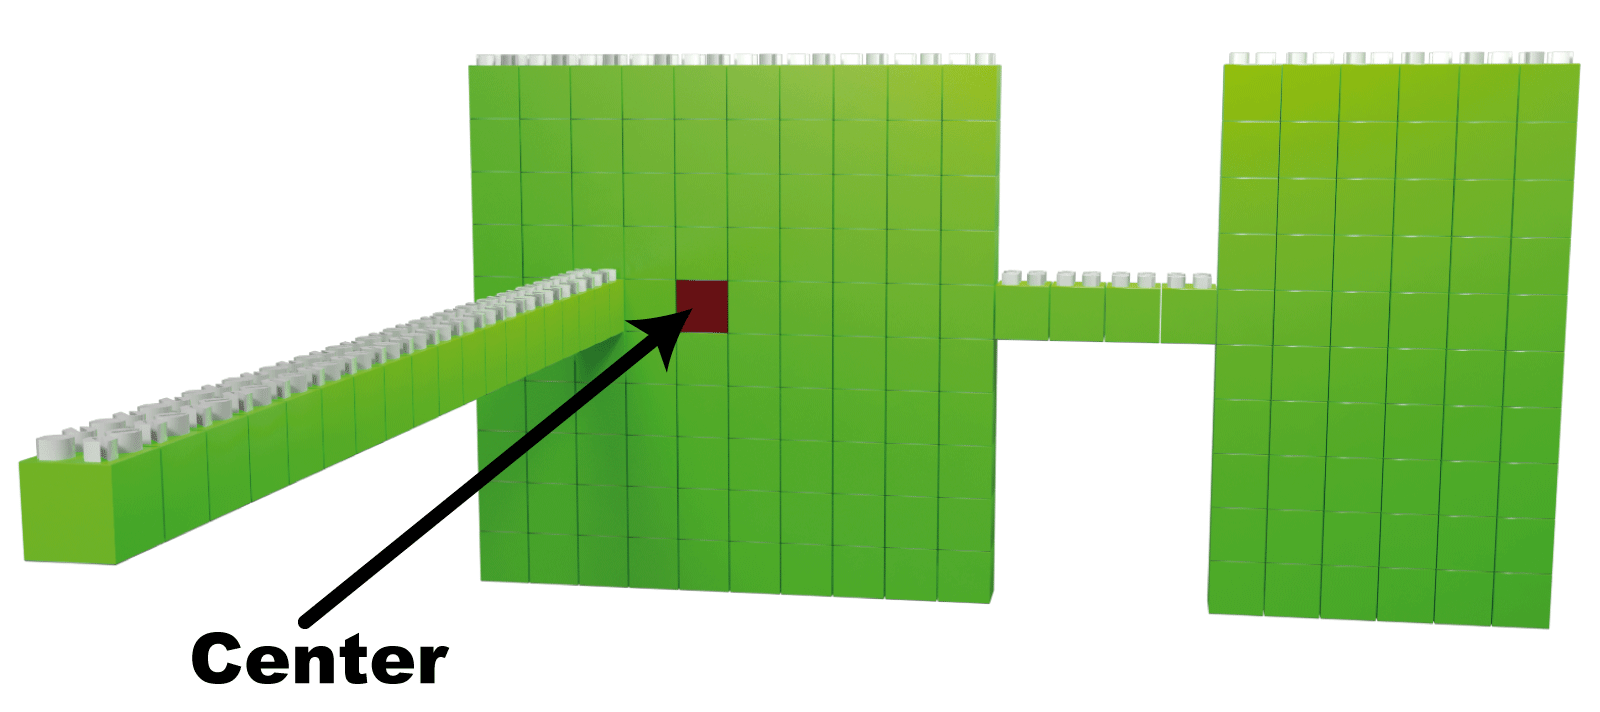
\includegraphics[height=0.35\paperheight]{fig/centrality/centers/center}
		\end{figure}
	\end{textblock*}
}

\only<5>{
	\begin{textblock*}{\paperwidth}(-0.5cm,0.57\paperheight)
		\begin{figure}
			\centering
			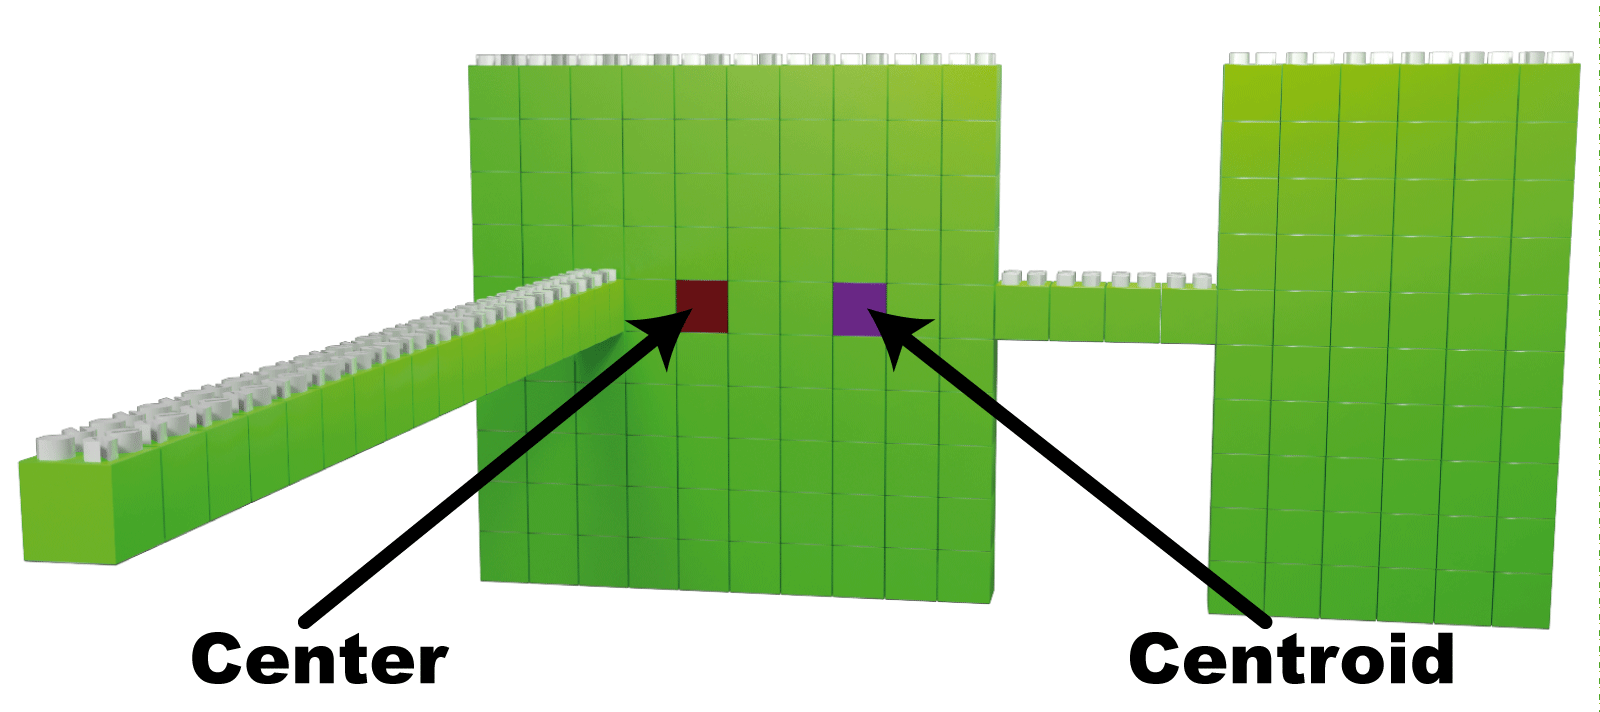
\includegraphics[height=0.35\paperheight]{fig/centrality/centers/center-centroid}
		\end{figure}
	\end{textblock*}
}

\end{frame}
}

\subsection{Related Work and Contributions}

\subsectionOutlineFrame

\noLogo{
\begin{frame} \frametitle{Related Work}
%TM vs decentralized
%clock skew compensation
{
	\footnotesize
	
	\newcommand{\lenTwo}{0.17\linewidth}
	\newcommand{\lenThree}{0.32\linewidth}
	\newcommand{\lenFour}{0.3\linewidth}

	\begin{center}
		\begin{tabular}{|C{\lenThree}|C{\lenTwo}|C{\lenTwo}|C{\lenTwo}|}
			\hline
			Approach & Accuracy (experiments) & Time and message cost & Memory cost\\ 
			\hline
			Naive and exhaustive (e.g., \cite{Korach:1984:DAF:579.585,mamei2005self}) & exact & +++++\hspace{2cm} (potential congestion) & + to +++++
			 \\
			\hline
			Graph specific (e.g., \cite{bruell1999self} for trees) & exact (but not for arbitrary graphs) & + & +\\
			\hline
			Approximation (e.g., \cite{wehmuth2013daccer, dissler2016distributed, kim2013leader}) & ++ to +++ & ++ & + to +++\\
			\hline
		\end{tabular}
	\end{center}

	Thesis contribution: %approximation algorithms for arbitrary networks
	\begin{center}
		\begin{tabular}{|C{\lenThree}|C{\lenTwo}|C{\lenTwo}|C{\lenTwo}|}
			\hline
			3 approximation algorithms & +++ to ++++ & +++ & + \\
			%(inspired from external- graph analysis methods)
			\hline
		\end{tabular}
	
	\remark{A good cost-accuracy trade-off}
	\end{center}


}

\end{frame}
}

\begin{frame} \frametitle{My Contributions}

\begin{itemize}
	\item 3 distributed algorithms:
	\begin{itemize}
		\item $k$-BFS SumSweep
		\item { ABC-Center} (two versions) %\bfseries
		\item Probabilistic Counter based Central Leader Election (PC2LE)
	\end{itemize}
	\item Inspired from existing external-graph analysis algorithms
	\item All based on intuitive heuristics
	\item Experimental evaluation of the accuracy
	\item Formal analysis of the performance:

{
	\scriptsize
	\newcommand{\lenOne}{0.12\linewidth}
	\newcommand{\lenFive}{0.17\linewidth}

\begin{center}
	\begin{tabular}{|C{\lenFive}|C{\lenOne}|C{\lenFive}|C{\lenFive}|C{\lenFive}|}
		\hline
		Name & Type of center & Time & Memory (per module) & Message\\
		\hline
		$k$-BFS SumSweep & center, centroid & $O(k\times d)$ & $O(\Delta)$ & $O(m \times n^2)$ \\
		\hline
		ABC-CenterV2 & center & O($\#steps \times d$) & $O(\Delta)$ & $O(m \times n^2)$ \\
		\hline
		PC2LE & center, centroid & O($d$) & $O(\Delta + $ $|$probabilistic counter$|)$ & $O(m \times n^2)$ \\
		\hline
	\end{tabular}
\end{center}
	Notation:\\
	$n = \# $modules, $m = \#$ links, $d = $ diameter, $\Delta = $ maximum number of neighbors\par
}
\end{itemize}

\end{frame}

\subsection{ABC-CenterV2}

\subsectionOutlineFrame

\subsubsection{General Idea}

\begin{frame} \frametitle{General Idea}

\begin{itemize}
	\item Extends the sequential MiniMax algorithm~\cite{handler1973minimax} for tree graphs
	\item Idea: the center stands at the middle of a diameter (i.e., longest path)
\end{itemize}

\begin{center}
	\begin{columns}[c]
	\begin{column}{.5\textwidth}
		\centering
		\adjincludegraphics[width=1\linewidth,valign=c]{fig/centrality/abc-centerv2/mid-diameter-4.png}
	\end{column}
	\begin{column}{.3\textwidth}
		\only<2> {
			\centering
			\adjincludegraphics[width=\linewidth,valign=c]{fig/centrality/twoSweep.png}
		}
	\end{column}
\end{columns}
\end{center}

\end{frame}

\subsubsection{Algorithm}

\begin{frame} \frametitle{Algorithm}

\begin{center}
\myAlg{
	{$Candidates\gets all\ modules$\;}
	
	\While{$|Candidates| > 2$}{
		
		{$A \gets v_i \in Candidates$;\ \tcp{A is a random candidate}}
		
		{$B \gets v_i \in \argmax\limits_{v_j \in Candidates} d(A, v_j)$;\ \tcp{B a farthest candidate from A}}
		
		{$C \gets v_i \in \argmax\limits_{v_j \in Candidates} d(B, v_j)$;\ \tcp{C a farthest candidate from B}}
				
		\tcp{Most equi-distant nodes from B to C remain candidate:}
		{$Candidates \gets  \argmin\limits_{v_j \in Candidates} |d(B,v_j) - d(C,v_j)| $\;}
	
		\tcp{\footnotesize B and C are eliminated (if not already purged by the previous line):}
		{$Candidates \gets Candidates - \{B, C\}$\;}
	}
	
	{$central \gets  v_i \in Candidates$;\ \tcp{a random candidate}}
}
\end{center}

Single-source shortest paths are computed using distributed breadth-first network traversals (based on~\cite{cheung1983graph}).

\end{frame}

\subsubsection{Examples}

\begin{frame} \frametitle{Examples - One-step 2D Shape}

\only<1> {
	\begin{figure}
		\centering
		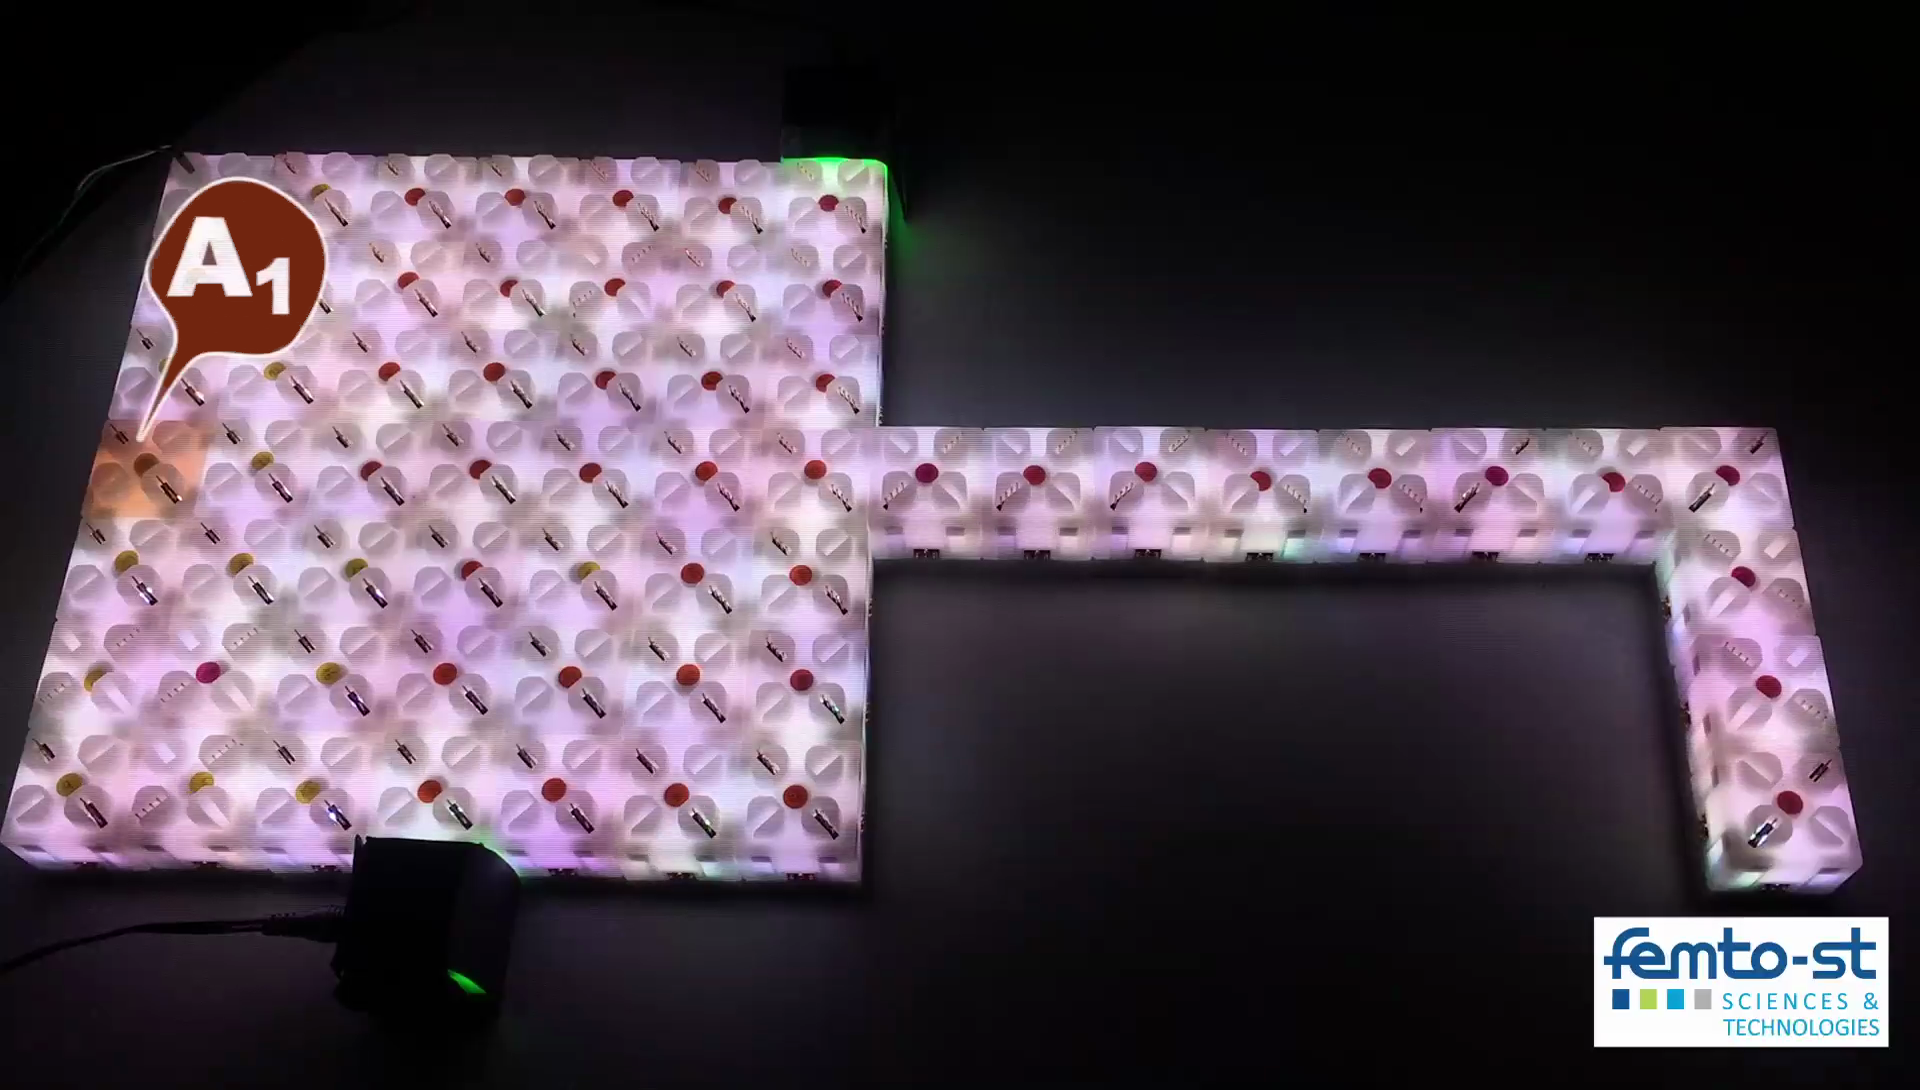
\includegraphics[width=0.7\linewidth]{fig/centrality/abc-center-example-2/1}
	\end{figure}
}

\only<2> {
	\begin{figure}
		\centering
		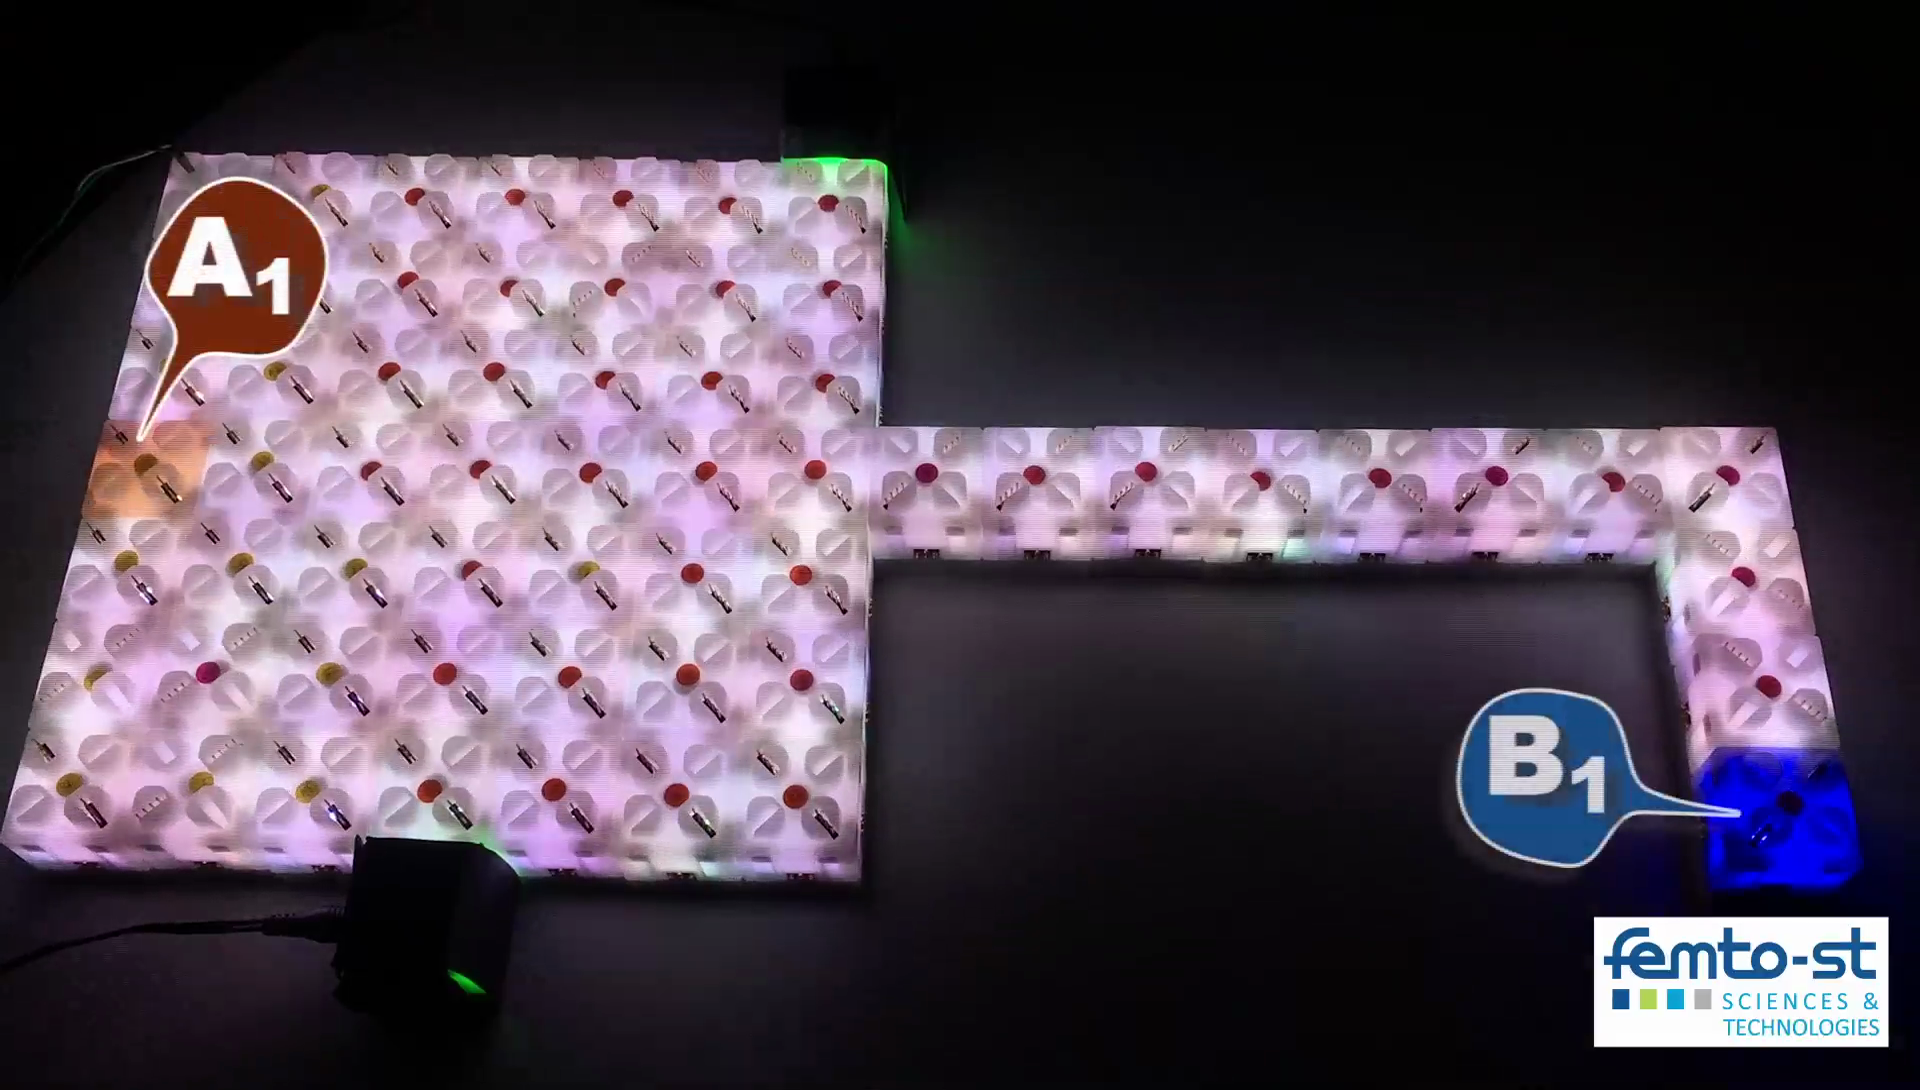
\includegraphics[width=0.7\linewidth]{fig/centrality/abc-center-example-2/2}
	\end{figure}
}

\only<3> {
	\begin{figure}
		\centering
		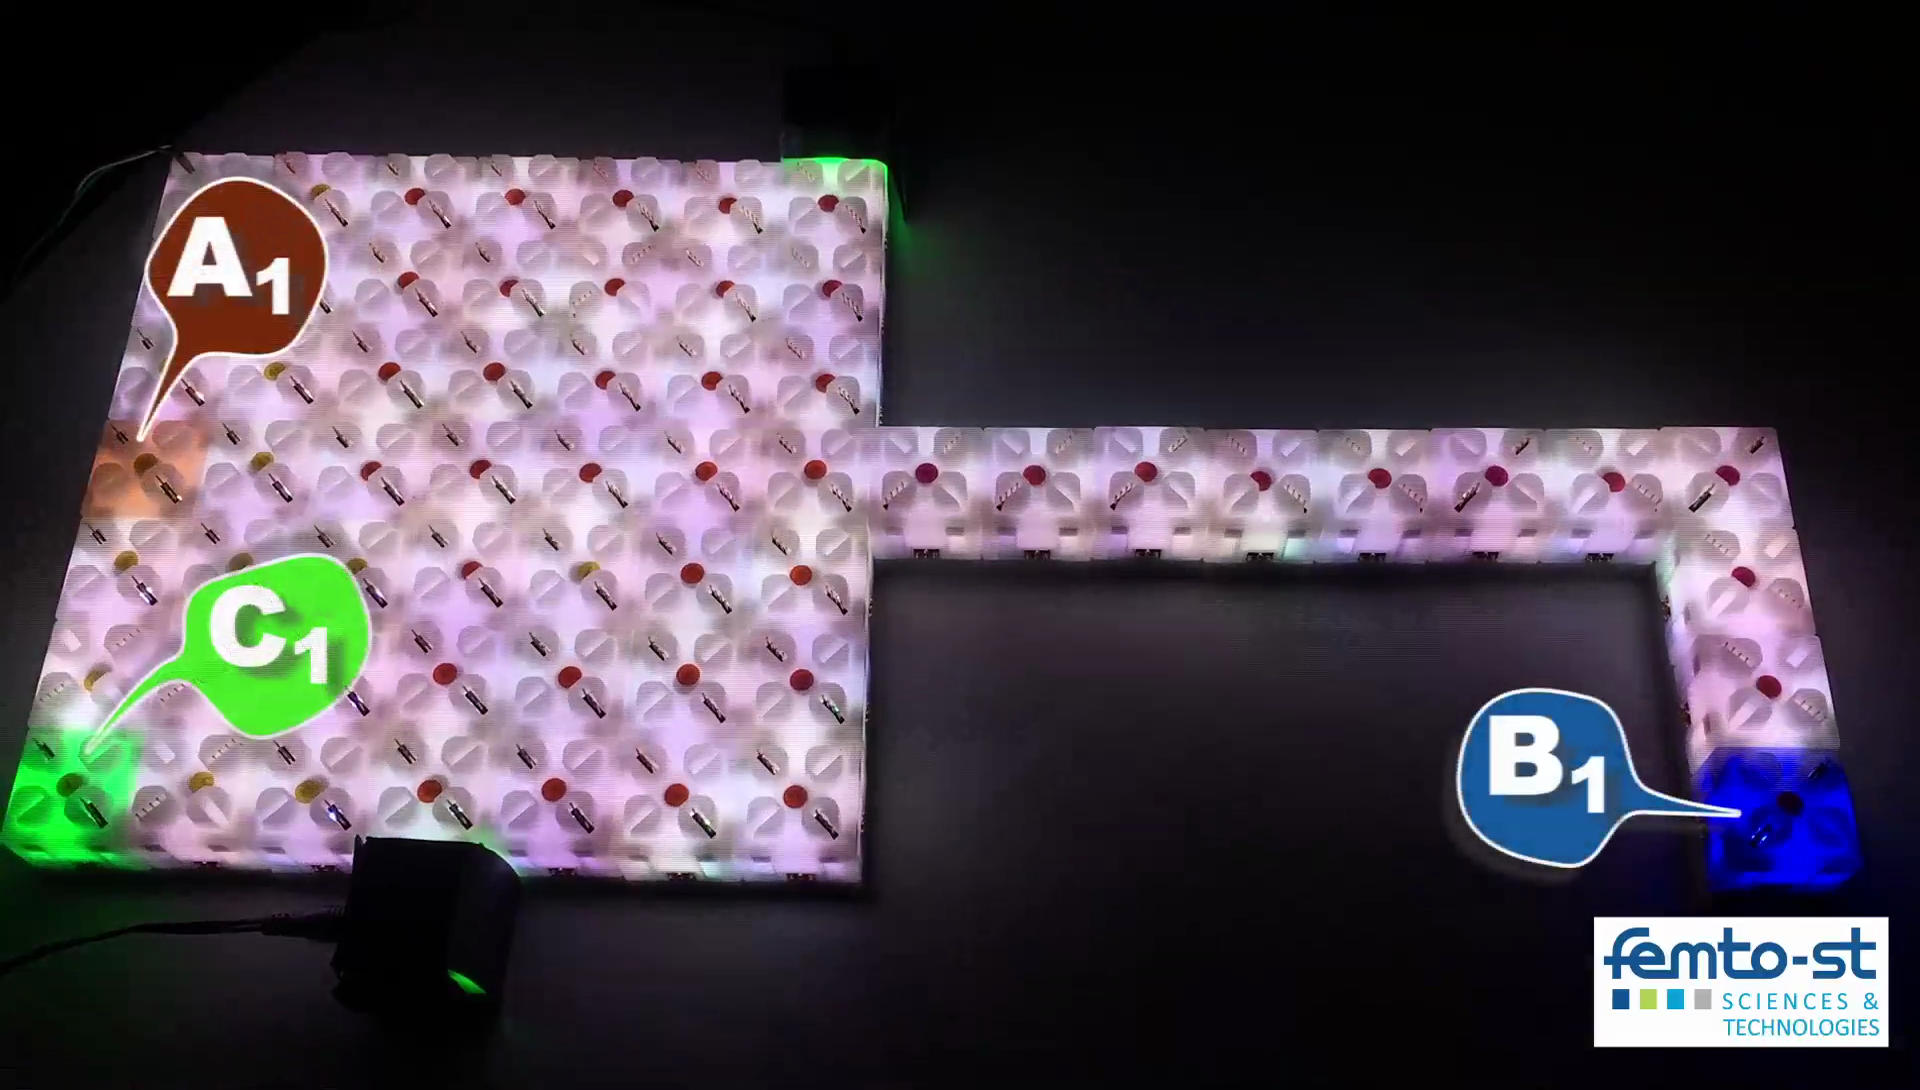
\includegraphics[width=0.7\linewidth]{fig/centrality/abc-center-example-2/3}
	\end{figure}
}

\only<4> {
	\begin{figure}
		\centering
		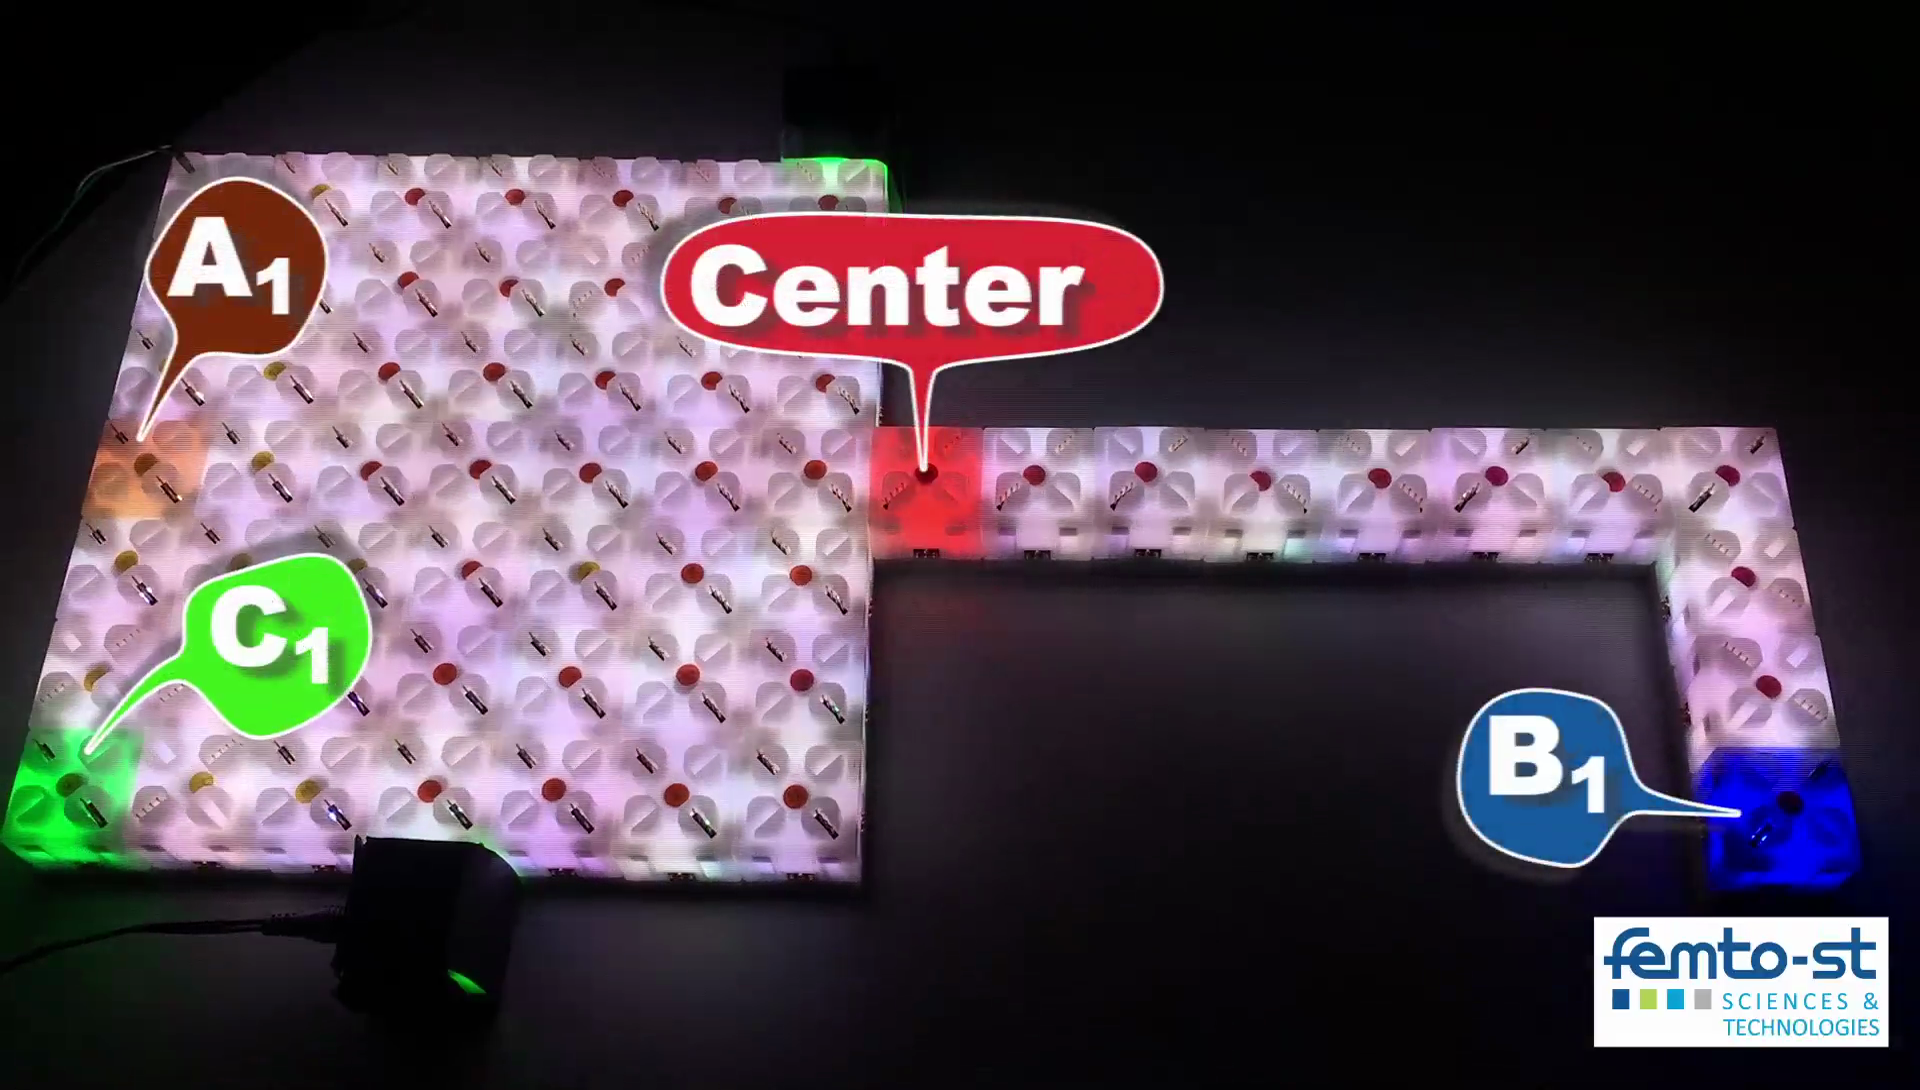
\includegraphics[width=0.7\linewidth]{fig/centrality/abc-center-example-2/4}
	\end{figure}
}

\begin{center}
	\vspace{-0.5cm}\hspace*{5cm}$^*$60 Blinky Blocks
\end{center}

\end{frame}

\begin{frame} \frametitle{Examples - More complex}
\vspace{1cm}
\begin{center}
\only<1> {
	\begin{figure}
		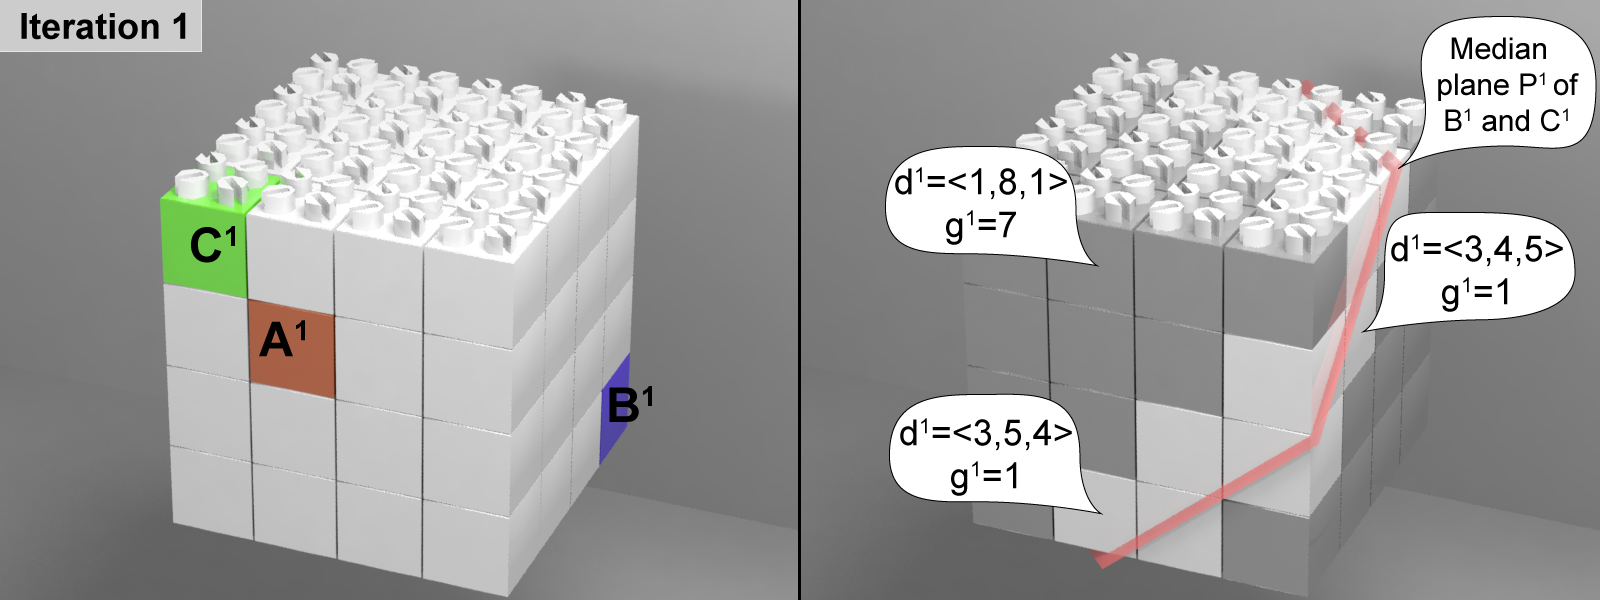
\includegraphics[width=\linewidth]{fig/centrality/abc-centerv2/cube/step1}
	\end{figure}
}

\only<2> {
	\begin{figure}
		\centering
		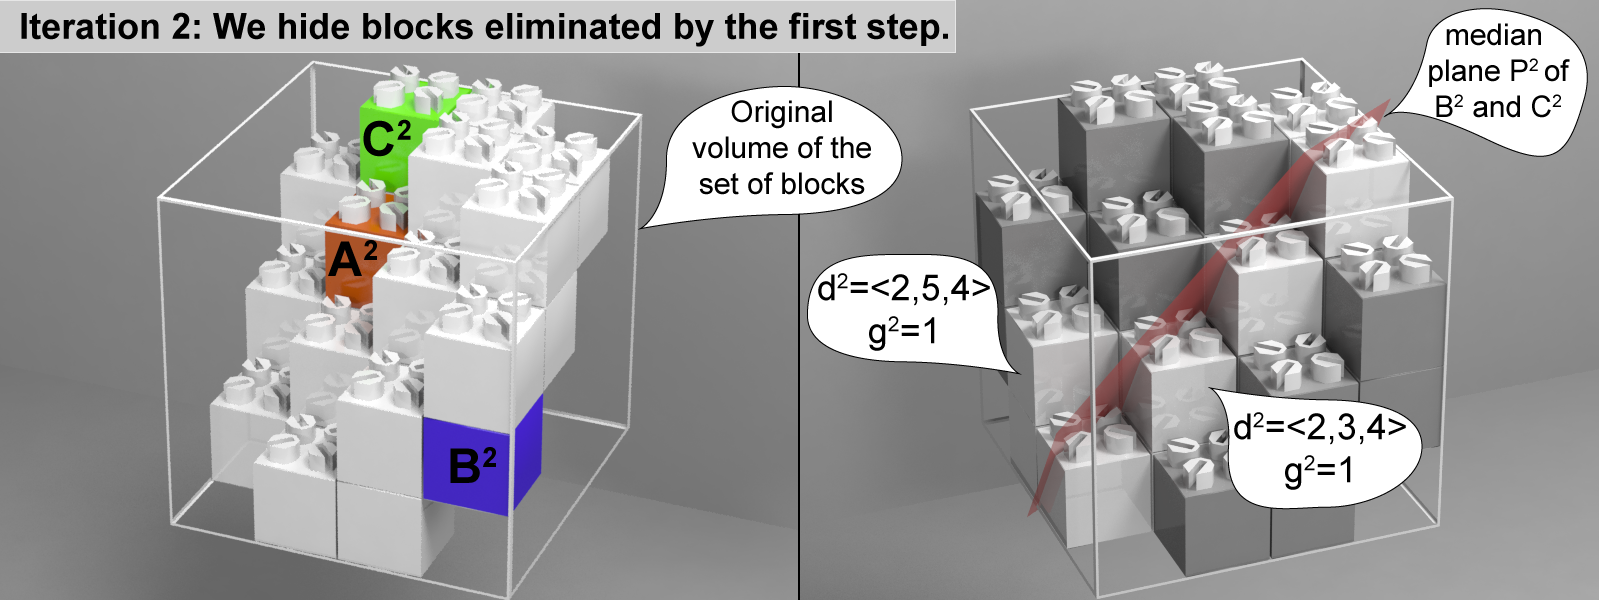
\includegraphics[width=\linewidth]{fig/centrality/abc-centerv2/cube/step2}
	\end{figure}
}

\only<3> {
	\begin{figure}
	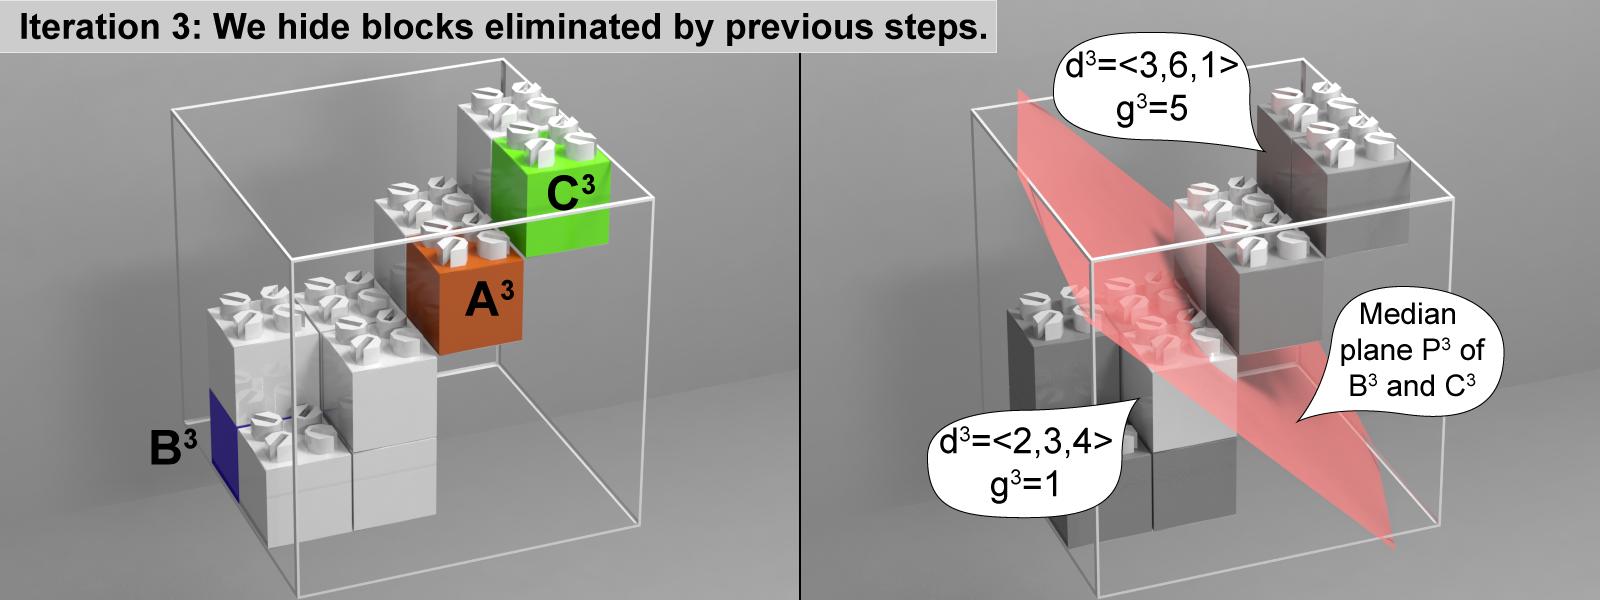
\includegraphics[width=\linewidth]{fig/centrality/abc-centerv2/cube/step3}
	\end{figure}
}

\only<4-> {
	\begin{figure}
		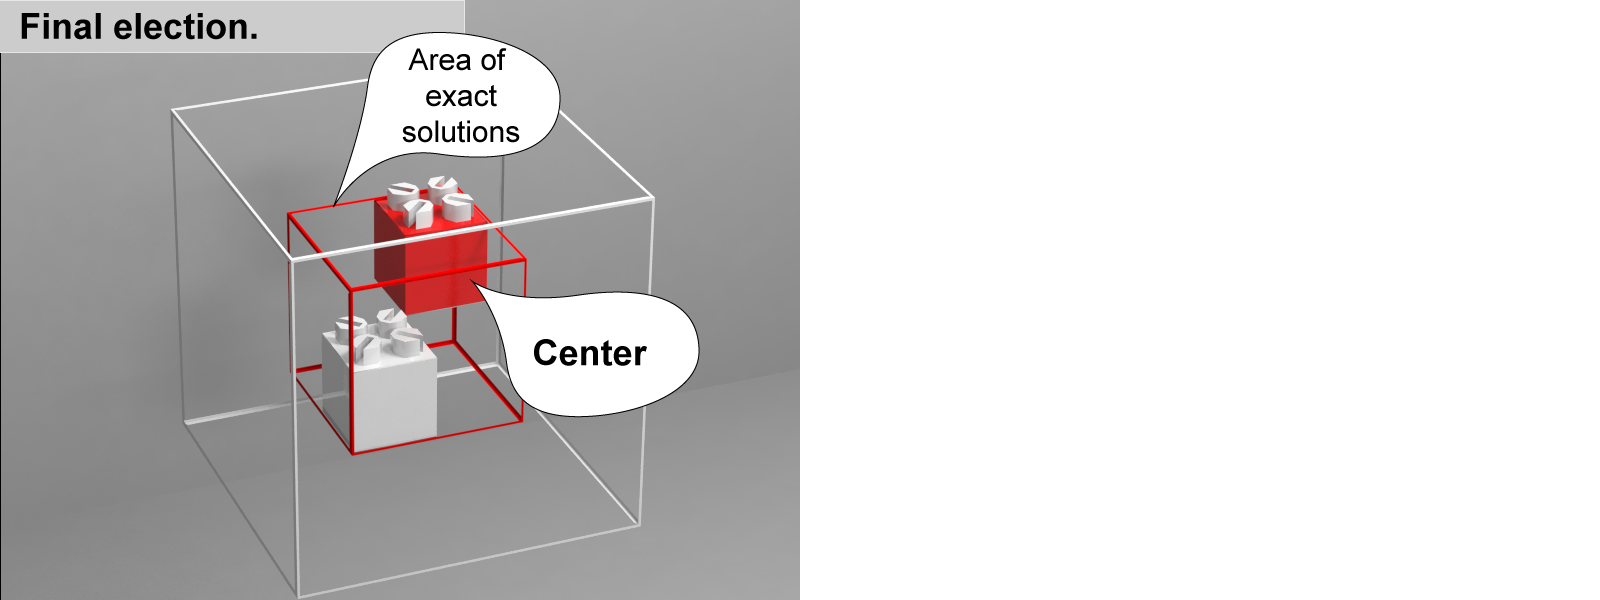
\includegraphics[width=\linewidth]{fig/centrality/abc-centerv2/cube/step4}
	\end{figure}
}
\end{center}

\only<5>{
	\remark{$\#$ steps increases with the thickness of the diameter}
	\remark{ABC-Center is more efficient in low-degree networks}
}
\end{frame}

\subsubsection{Tricky Case}

\begin{frame} \frametitle{Tricky Case for Future Work}
\begin{center}
	\begin{columns}[T]
		\begin{column}{.45\textwidth}
			\centering
			\adjincludegraphics[width=\linewidth]{fig/centrality/tricky-case/abc-center.png}
			ABC-CenterV1/V2
		\end{column}
		\begin{column}{.45\textwidth}
			\only<2-> {
				\centering
				\adjincludegraphics[width=\linewidth]{fig/centrality/tricky-case/trial.png}
				Envisioned but abandoned approach
			}
		\end{column}
	\end{columns}

\only<3> {
	\vspace*{0.5cm}
\remark{The envisioned approach solves this case but leads to less accuracy in experiments with random systems}

\remark{This specific case should be investigated in future work!}
}

\end{center}
\end{frame}

\subsection{Evaluation}

\subsectionOutlineFrame

\subsubsection{ABC-CenterV1 on Hardware}

\noLogo{
\begin{frame} \frametitle{ABC-CenterV1 on Hardware}

	\begin{figure}
	\centering
	\href{run:videos/21-abccenter-dynamics.avi?autostart&loop}{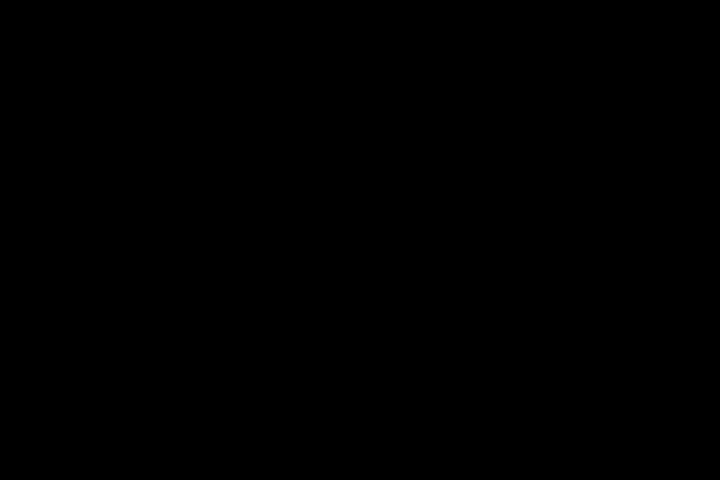
\includegraphics[width=0.7\textwidth]{videos/21-abccenter-dynamics.jpg}}
	\end{figure}

\end{frame}
}

\subsubsection{Simulation Fidelity}

\noLogo{
\begin{frame} \frametitle{VisibleSim Simulator Fidelity}

Statistical simulation model based on measurements
\begin{itemize}	
	\item Processing time
	\item Communication time
\end{itemize}

	{
		
		\newcommand{\vsfid}[1]{rien}
		\newcommand{\lenOneOne}{0.07\linewidth}
		\newcommand{\lenTwoTwo}{0.12\linewidth}
		\newcommand{\lenThreeThree}{0.15\linewidth}
		\newcommand{\lenFourFour}{0.2\linewidth}
		\begin{table}[!h]
			\centering			
			\small
			\begin{tabular}{|C{\lenTwoTwo}|C{\lenTwoTwo}|C{\lenThreeThree}|C{\lenThreeThree}|C{\lenFourFour}|}
				\hline
				& & \multicolumn{2}{c|}{average ABC-CenterV1} &  \\
				Shape & Size & \multicolumn{2}{c|}{execution time} &  \textcolor{\remarkColor}{Relative average}   \\
				 &  (module) & \multicolumn{2}{c|}{$\pm$ standard-deviation (ms)}& \textcolor{\remarkColor}{simulation} \\
				\cline{3-4}
				&  & Hardware & Simulator & \textcolor{\remarkColor}{precision}\\
				\hline
				\multirow{3}{*}{Line}  & 5 & $234 \pm 1$ & $244 \pm 3$ & \textcolor{\remarkColor}{95.7\%} \\
				%529611
				\cline{2-5}
				& 10 & $545 \pm 5$ & $544 \pm 5$ & \textcolor{\remarkColor}{99.8\%}\\
				%529611
				\cline{2-5}
				& 50 & $2873 \pm 23$ & $2885 \pm 17$ & \textcolor{\remarkColor}{99.6\%}\\
				%2879659
				\hline
				\multirow{3}{*}{Square} & 9 & $598 \pm 45$ & $588 \pm 14$ & \textcolor{\remarkColor}{98.3\%}\\
				\cline{2-5}
				& 25 & $1117 \pm 30$ & $1119 \pm 27$ & \textcolor{\remarkColor}{99.8\%}\\
				\cline{2-5}
				& 49 & $1684 \pm 48$ & $1686 \pm 44$ & \textcolor{\remarkColor}{99.9\%} \\
				% sim: 1646128
				\hline
				\multirow{2}{*}{Cube} & 27 &$ 1229 \pm 56$ & $ 1214 \pm 31$ & \textcolor{\remarkColor}{98.8\%} \\
				\cline{2-5}
				& 64 & $1927 \pm 51$ & $1941 \pm 33$ & \textcolor{\remarkColor}{99.3\%} \\
				\hline
				Dumbbell & 59 & $1262 \pm 56$ & $1252 \pm 57$& \textcolor{\remarkColor}{99.2\%} \\
				\hline
			\end{tabular}
		\end{table}
	}

\remark{VisibleSim accurately simulates our algorithm on the Blinky Blocks}
	
\end{frame}
}

\subsubsection{Simulation Evaluation}

\newcommand{\ResultsScaleFactor}{1}

\begin{frame} \frametitle{Simulation Evaluation}

\begin{itemize}
	\item Simulations using VisibleSim
	\item Comparisons with other algorithms
	\begin{itemize}
		\item Random: MIN-ID~\cite{raynal2013distributed}
		\item Exhaustive: BARYCENTER~\cite{mamei2005self}
		\item Approximations:
		\begin{itemize}
			\item  TBCE~\cite{kim2013leader}
			\item  $k$-BFS-RAND, our distributed version of~\cite{eppstein2001fast}
			\item PC2LE with \cite{garin2012distributed} 's probabilistic counter
		\end{itemize}
	\end{itemize}
	\item Systems
	\begin{itemize}
		\item Random compact shapes
		%: randomly connecting\\modules one-by-one starting from a\\ single module.
		\item Different sizes: 10 to 25,000 modules
		\item Statistics on multiple independent\\runs
	\end{itemize}
	\item Evaluation criteria
	\begin{itemize}
		\item Accuracy
		\item Cost
		\begin{itemize}
			\item Execution time
			\item Number of messages
			\item Memory usage
		\end{itemize}
	\end{itemize}
	\end{itemize}

\begin{textblock*}{0.39\paperwidth}(0.6\paperwidth,0.45\paperheight)
	
	\begin{figure}
		\centering
		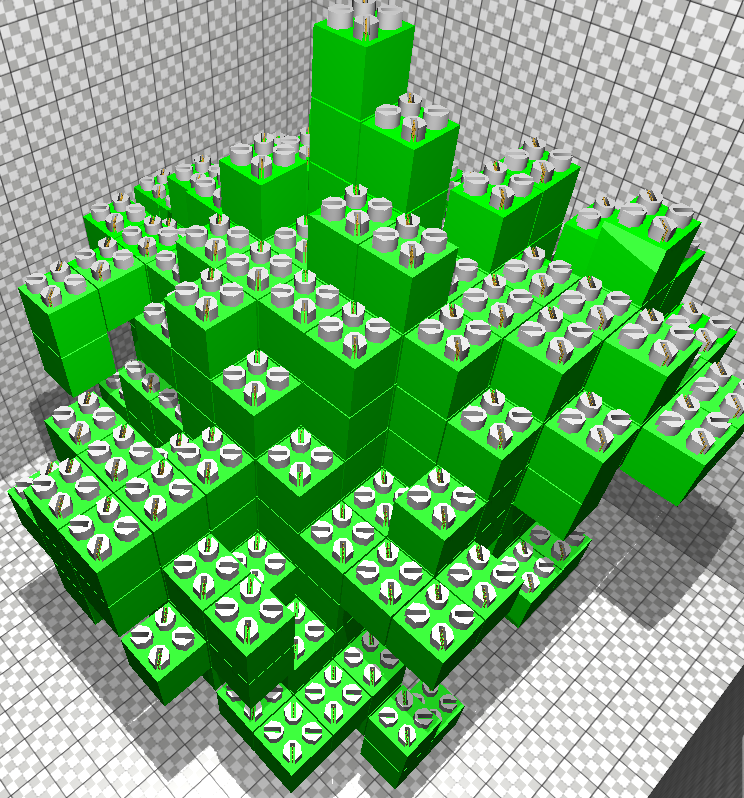
\includegraphics[width=0.8\linewidth]{fig/centrality/random-500modules}
	\end{figure}
\end{textblock*}
\end{frame}

\noLogo{
\begin{frame} \frametitle{Relative accuracy}

{
	\small
	\begin{align*}
	relative\ center\ accuracy = 1 - \left|\frac{ecc(center)- ecc(elected\ node)}{ecc(center)}\right|
	\end{align*}
}
\vspace{-0.25cm}
\begin{figure}
	\centering
	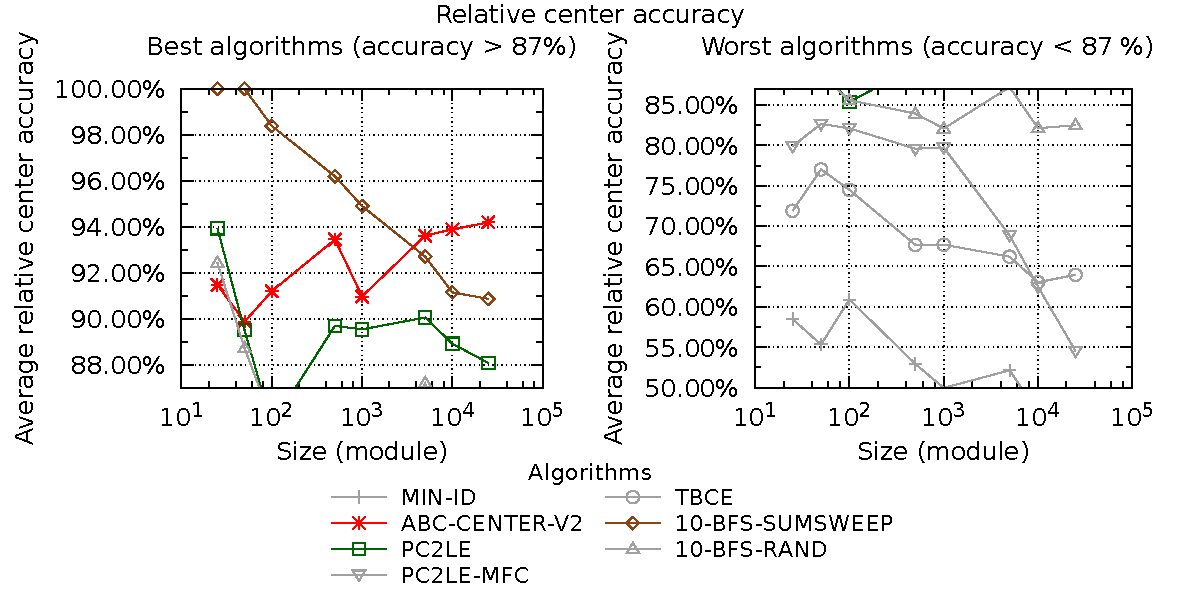
\includegraphics[width=0.825\linewidth]{fig/centrality/accuracy-center}
\end{figure}

\remark{Our algorithms:\\most precise approximation algorithms (accuracy $> 85\%$)}

\end{frame}
}

\begin{frame} \frametitle{Execution Time}

\begin{center}
	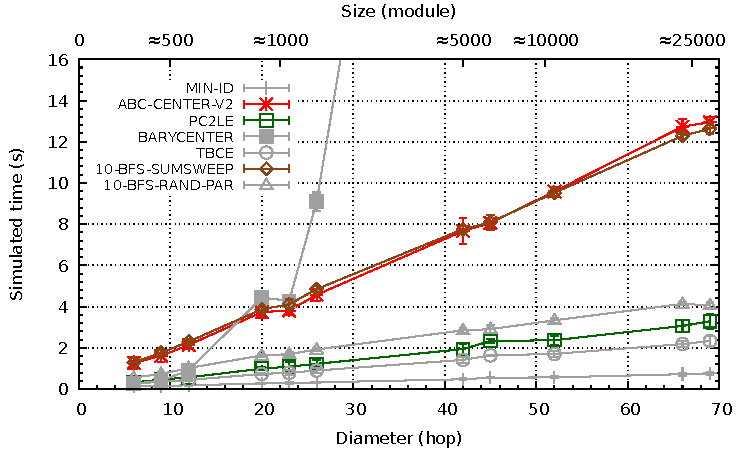
\includegraphics[width=0.9\linewidth]{fig/centrality/time}
\end{center}
\remark{A good trade-off between cost and accuracy}
\end{frame}


\begin{frame} \frametitle{Average number of messages per module}
\begin{center}
	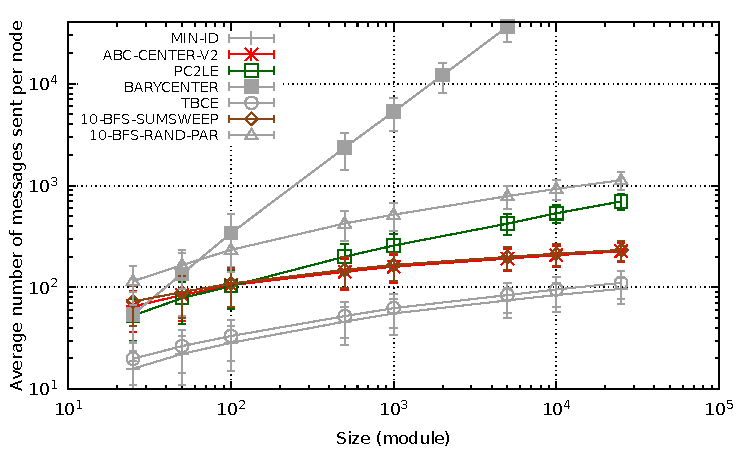
\includegraphics[width=0.9\linewidth]{fig/centrality/avgMessages}
\end{center}

\remark{A good trade-off between cost and accuracy}
\end{frame}


\begin{frame} \frametitle{Memory usage}

\begin{figure}
	\centering
	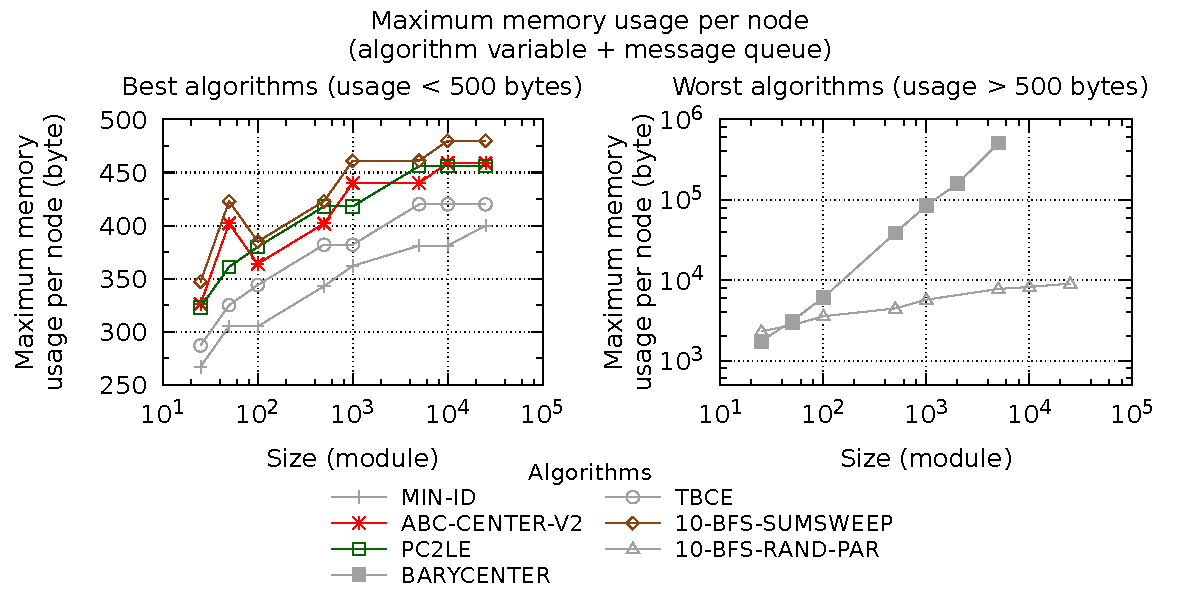
\includegraphics[width=0.9\linewidth]{fig/centrality/memory-defense}
\end{figure}

\remark{Our algorithms have a bounded and limited memory usage\\($< 500$ bytes per module)}

\end{frame}

\subsection{Conclusion}

\begin{frame} \frametitle{Conclusion}

\begin{itemize}
	\item 3 efficient distributed centrality-based leader election algorithms
		\begin{itemize}
			\item $k$-BFS SumSweep, ABC-Center and PC2LE
		\end{itemize}
	\item Robustness to network dynamics
	\item Formal analysis of the performance (time, message and memory)
	\item Evaluation
		\begin{itemize}
			\item Hardware: 5 to 64 modules
			\item Simulations: 10 to 25,000 modules
			\begin{itemize}
				\item Most precise approximation algorithms ($> 85\%$ relative center accuracy)
				\item Good cost-accuracy trade-off 
			\end{itemize}
		\end{itemize}
	\item Limits
		\begin{itemize}
			\item Experimental evaluation of the accuracy
			\item Bad cases?
			\item Efficiency in other platforms with different network structures?
				\begin{itemize}
					\item Our algorithms: inspired from external-graph analysis algorithms used to study large-scale real-world networks (e.g., YahooWeb, AS networks)
				\end{itemize}
		\end{itemize}
\end{itemize}
\end{frame}

\section{Time Synchronization}

\subsection{Problem and Motivation}

\begin{frame} \frametitle{Problem}
  \begin{itemize}
    \item Problem: maintain a global timescale through the system 
	\begin{figure}
	\centering
	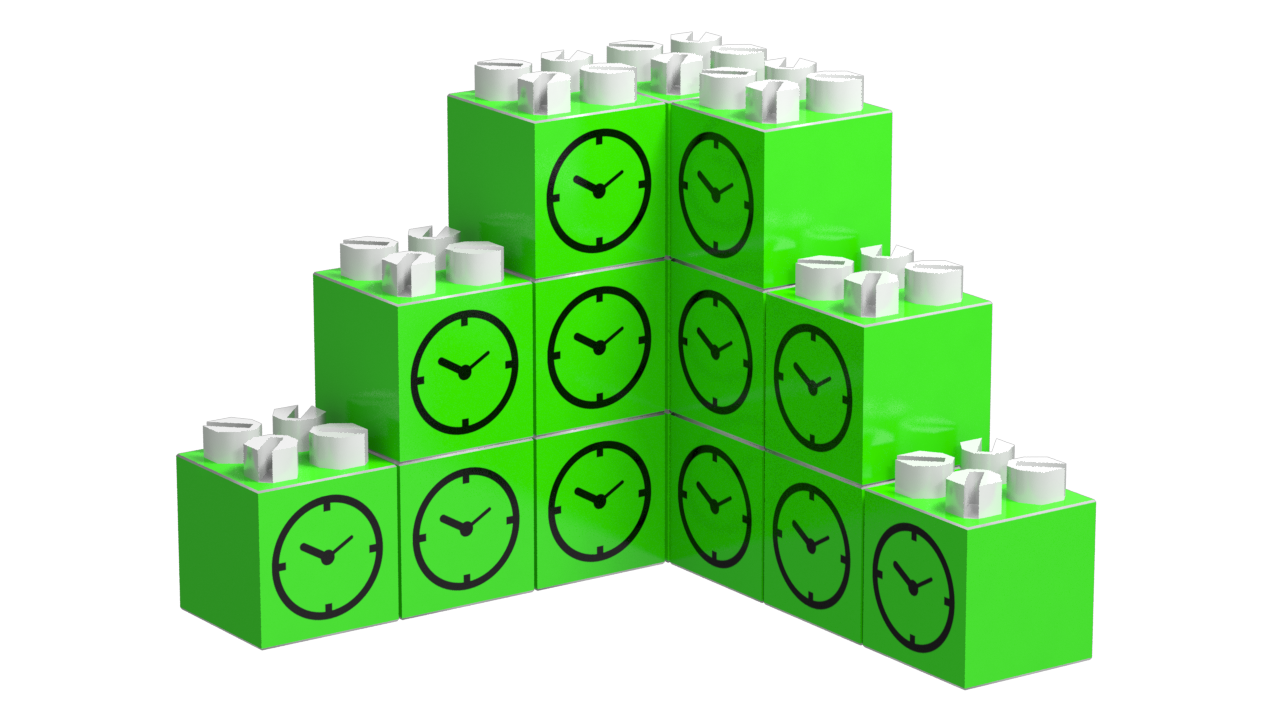
\includegraphics[height=0.325\paperheight]{fig/synchronization/clock-bb-illustration.png}
	\end{figure}
    \item Challenges:
      \begin{itemize}
      \item Imperfect hardware clocks (clock drift, skew, offset and noise)
      \item Handling communication delays
      \end{itemize}
 \end{itemize}
\end{frame}

\noLogo{
\begin{frame} \frametitle{Motivation}

Distributed coordination (e.g., distributed bitmap scroller)

\begin{center}	
	\begin{columns}[c]
		\begin{column}{.5\textwidth}
		\centering
		\href{run:videos/31-scroller-goal.avi?autostart&loop}{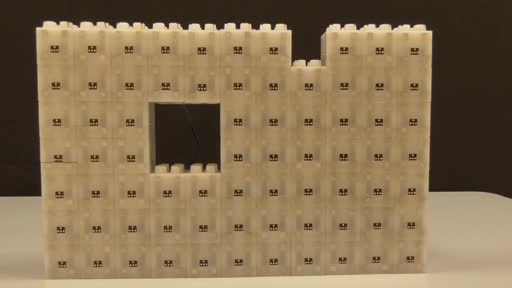
\includegraphics[width=0.95\linewidth]{videos/31-scroller-goal.jpg}}
		\end{column}
		\begin{column}{.5\textwidth}
		\centering			
		72-Blinky-Blocks scroller synchronized with our protocol (MRTP)
		\end{column}
	\end{columns}
\end{center}

Unsynchronized scroller:
\begin{center}	
\begin{columns}[c]
	\begin{column}{.33\textwidth}
		\centering
		Start:\\
		\href{run:videos/31-unsync1.avi?autostart&loop&start=1}{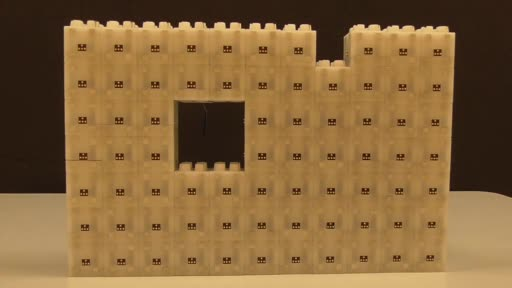
\includegraphics[width=0.9\linewidth]{videos/31-unsync1.jpg}}
	\end{column}
	\begin{column}{.33\textwidth}
		\centering
		1min20:\\
		\href{run:videos/31-unsync2.avi?autostart&loop}{
\includegraphics[width=0.95\linewidth]{videos/31-unsync2.jpg}}
	\end{column}  
	\begin{column}{.33\textwidth}
		\centering
		20min:\\
		\href{run:videos/31-unsync3.avi?autostart&loop}{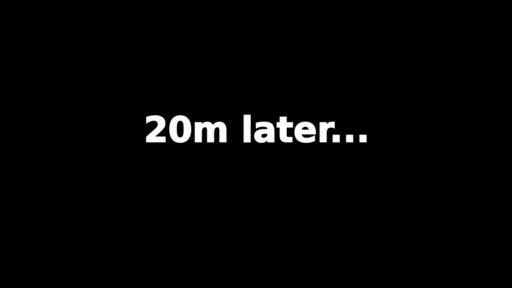
\includegraphics[width=0.95\linewidth]{videos/31-unsync3.jpg}}
	\end{column} 
\end{columns}
\end{center}
\vspace{-0.35cm}
\remark{This application requires a global timescale}
\end{frame}
}

\subsection{Assumptions}

\begin{frame}\frametitle{Assumptions}

Illustrated on the Blinky Blocks modular robot, but suitable for networked embedded devices with:

	\begin{itemize}
		%\item Non-anonymous (unique identifiers used for leader election)
    	\item Local clocks
    		\begin{itemize}
    			\item Nearly identical precision/resolution (potentially poor)
    				\begin{itemize}
    					\item Blinky Blocks: 1\% precision, 1 ms resolution
    				\end{itemize}
    		%	\item Quasi-linear skew
    		\end{itemize}
    	\item Network
    	    \begin{itemize}
    	    	%\item Undirected and unweighted 
    	    	\item Neighbor-to-Neighbor communications
    	    	\item Potentially: large network size and large diameter
    	    	\item Fairly stable
    	    	%\item Low-level timestamping mechanism
    	    \end{itemize}
    \end{itemize}

\begin{center}
\begin{columns}[c]
	\begin{column}{.5\textwidth}
		\centering
		Split:\\
		\href{run:videos/32-split.avi?autostart&loop}{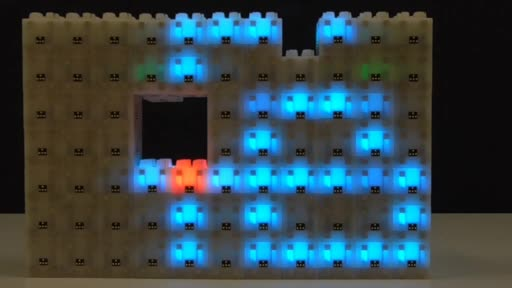
\includegraphics[width=0.9\linewidth]{videos/32-split.jpg}}
	\end{column}
	\begin{column}{.5\textwidth}
		\centering
		Merge (after 2 hours):\\
		\href{run:videos/32-merge.avi?autostart&loop}{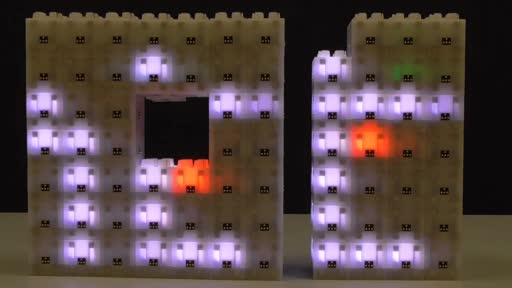
\includegraphics[width=0.9\linewidth]{videos/32-merge.jpg}}		
	\end{column} 
\end{columns}
\end{center}

\end{frame}

\subsection{Related Work}

\noLogo{
\newcommand{\lenMinusOne}{0.08\linewidth}
\newcommand{\lenZero}{0.08\linewidth}
\newcommand{\lenOne}{0.12\linewidth}
\newcommand{\lenTwo}{0.16\linewidth}
\newcommand{\lenThree}{0.20\linewidth}
\newcommand{\lenFour}{0.15\linewidth}
\begin{frame} %[shrink=2]
  \frametitle{Related Works}

\vspace{-0.25cm}
\tiny
\begin{center}
	\begin{tabular}{|C{\lenFour}|C{\lenZero}|C{\lenTwo}|C{\lenMinusOne}|C{\lenThree}|C{\lenOne}|}
	\hline
	Name &  Domain & Architecture & Infrastructure & Synchronization Technique & Clock Skew Compensation\\
	\hline
	NTP \cite{mills1991internet} & \multirow{4}{\linewidth}{\centering Computer Networks} & Master/Slave Master(s): pre-configured & \multirow{4}{\linewidth}{\centering Tree} & (Multi-hop) round-trip messages with frame-level timestamps and statistics & Phase/frequency locked loops \\
	\cline{1-1}
	\cline{3-3}
	\cline{5-6}
	PTP \cite{ptp2008} & & Master/slave Master: best clock & & Round-trip with low-level timestamps and per-hop delay compensation & \\
	\hline
	RBS \cite{elson2002fine} & \multirow{15}{\linewidth}{\centering Sensor Networks} & Master/Slave & Clustering  & Reference broadcast  & \multirow{15}{\linewidth}{\centering Linear model} \\
	\cline{1-1}
	\cline{3-5}	
	ATS [Schenato et al., 2011] &  & \multirow{4}{\linewidth}{\centering Fully distributed} & \multirow{4}{\linewidth}{\centering /} & Average-based consensus. Byte-level timestamps &  \\
	% \cite{schenato2011average}
	\cline{1-1}
	\cline{5-5}
	MTS \cite{he2014time,he2014study} &  &  & & Extremum-value based consensus. Byte-level timestamps & \\
	\cline{1-1}
	\cline{3-5}
	TPSN + MLE \cite{leng2010clock} &  & Master/slave & Tree & Recursive per-hop synchronization. Round- trip with frame-level timestamps and statistics & \\
	\cline{1-1}
	\cline{3-5}
	FTSP \cite{maroti2004flooding} &  & \multirow{5}{\linewidth}{\centering Master/slave Master: minimum-id implicit election} &  \multirow{4}{\linewidth}{\centering /} & Periodic asynchronous broadcasts. Byte-level timestamps and statistics &  \\
	\cline{1-1}
	\cline{5-5}			
	PulseSync \cite{lenzen2015pulsesync} &  & & & Fast flooding using broadcast. Byte-level timestamps & \\
	\hline
	\end{tabular}
\end{center}

\begin{center}
	\begin{tabular}{|C{\lenFour}|C{\lenZero}|C{\lenTwo}|C{\lenMinusOne}|C{\lenThree}|C{\lenOne}|}
	\hline
	Contribution: MRTP  & \textcolor{\remarkColor}{Modular Robotic} & Master/Slave  \textcolor{\remarkColor}{Master: central} & \textcolor{\remarkColor}{Breadth- first} spanning- tree &  Fast recursive per-hop synchronization. \textcolor{\remarkColor}{Compensation comm. delays: best for target system} & Linear model\\
	\hline
	\end{tabular}
\end{center}
\end{frame}
}

\subsection{Contribution: The Modular Robot Time Protocol (MRTP)}

\subsectionOutlineFrame

\subsubsection{Workflow}
\begin{frame} \frametitle{Contribution: The Modular Robot Time Protocol (MRTP)}
\begin{center}
    \begin{columns}[t]
      \begin{column}{.80\textwidth}
		\begin{enumerate}
			\item Initialization
			\begin{enumerate}
			\item Central time master election
			%(e.g., ABC-Center, $k$-BFS SumSweep, PC2LE)
			\item Breadth first spanning-tree construction
			%\item Set all clocks to the maximum global clock
			\end{enumerate}
			\item Periodic synchronization
			\begin{itemize}
				\item Best-suited method to compensate for\\communication delays
				\item Clock skew compensation using linear regression
			\end{itemize}
		\end{enumerate}
      
      ~\\
      $G(t)$: global time, held by the time master\\
      $\tilde{G}(t)$: disseminated estimation of $G(t)$
      
      \end{column}
      \begin{column}{.20\textwidth}
		\begin{figure}
			\centering
			\hspace{-1cm}
			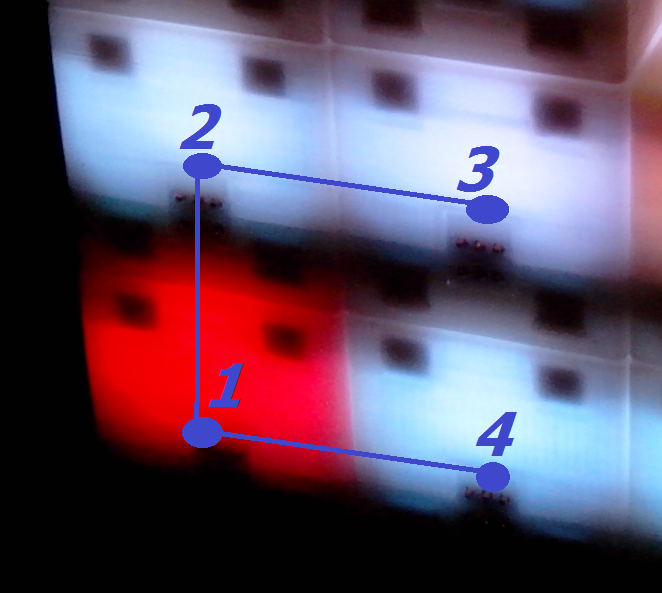
\includegraphics[width=1.25\linewidth]{fig/synchronization/sub-system}\\~\\
			\vspace*{-0.25cm}
			\hspace*{-3cm}
			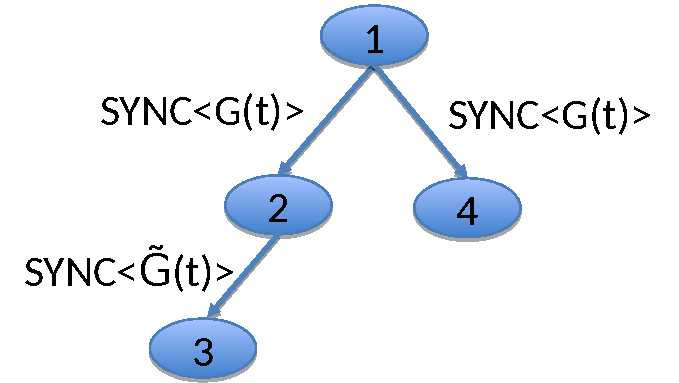
\includegraphics[width=2.3\linewidth]{fig/synchronization/tree}
			\label{fig:sub-system}
		\end{figure}
      \end{column}
  \end{columns}
  \end{center}
\end{frame}

\subsubsection{The Predictive Method to Compensate for Communication Delays}

\begin{frame} \frametitle{The Predictive Method to Compensate for Communication Delays}

\begin{figure}
	\centering
	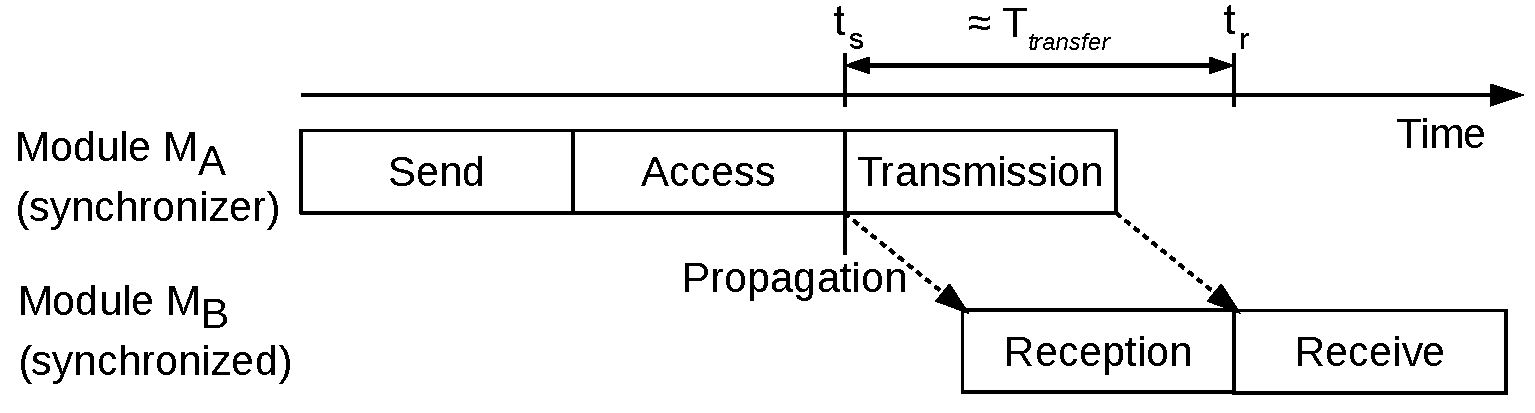
\includegraphics[width=0.75\linewidth]{fig/synchronization/synchronization-timestamp}
	\label{fig:synchronization-timestamp}
\end{figure}

\begin{figure}
	\centering
	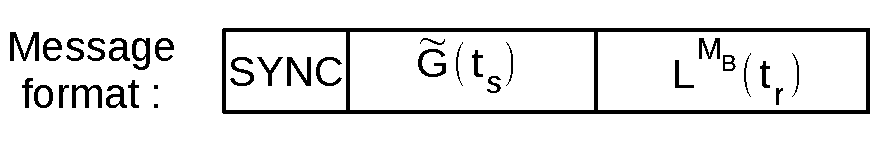
\includegraphics[width=0.5\linewidth]{fig/synchronization/synchronization-message}
	\label{fig:synchronization-message}
\end{figure}

\begin{center}
	\[
	\tilde{G}(t_r) = \tilde{G}(t_s) + T_{transfer}
	\]
	Linear regression on a window of synchronization points $<\tilde{G}(t),L^{M_B}(t)>$
	\[
	G^{M_B}(t) = a^{M_B}(t) * L^{M_B}(t) + b^{M_B}(t)
	%\forall t, \forall t', t \geq t', \ G^{M_B}(t) = max(G^{M_B}(t'),\ a^{M_B}(t)*L^{M_B}(t) + b^{M_B}(t))
	\]
\end{center}

\end{frame}

\subsection{Evaluation}

\subsectionOutlineFrame

\subsubsection{Blinky Blocks: Compensation for Communication Delays?}

\begin{frame}\frametitle{The Blinky Blocks Communication delays}

\begin{center}
	\begin{columns}[c]
		\begin{column}{.50\textwidth}
			\begin{figure}
				\centering
				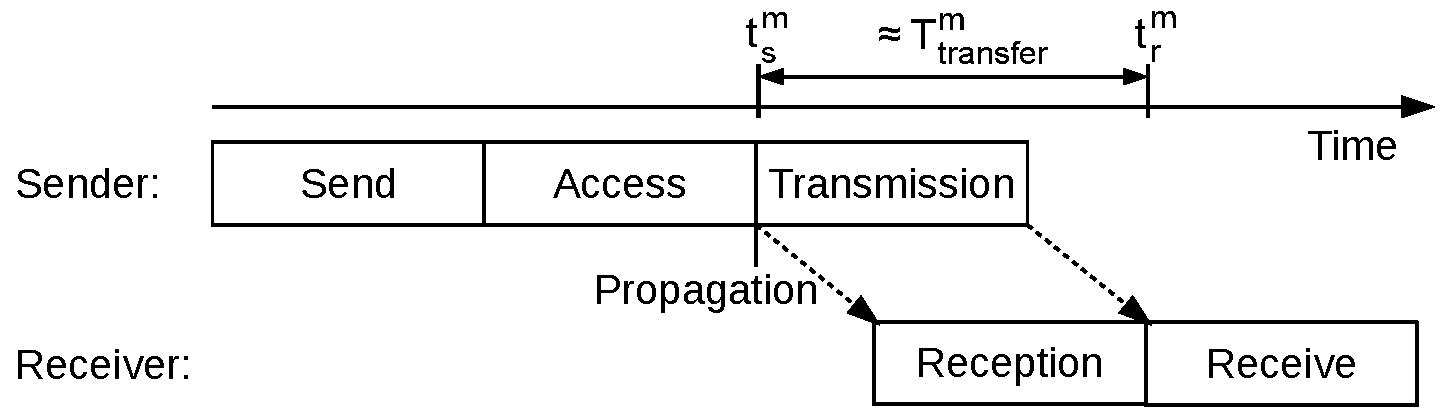
\includegraphics[width=\linewidth]{fig/synchronization/network-delay}
				\label{fig:communication-delays}
			\end{figure}
		\end{column}
		\begin{column}{.50\textwidth}
			\begin{figure}
				\centering
				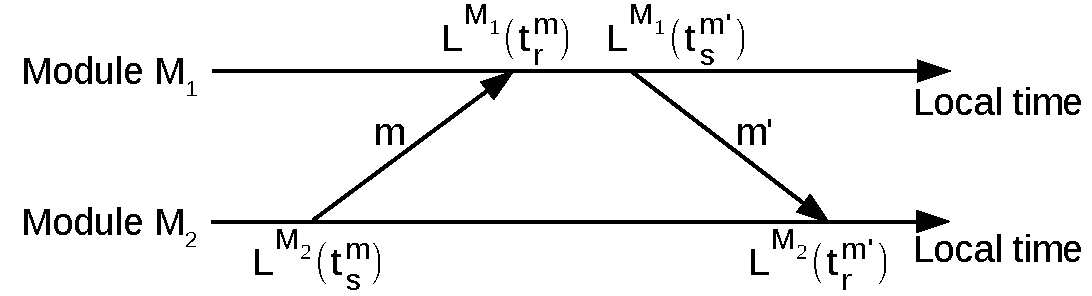
\includegraphics[width=\linewidth]{fig/synchronization/two-way}
				\label{fig:two-way}
			\end{figure}
			
		\end{column}
	\end{columns}
\end{center}

{
	\[ T_{transfer} \approx \frac{(L^{M_2}(t_r^{m'}) - L^{M_2}(t_s^m)) - (L^{M_1}(t_s^{m'})-L^{M_1}(t_r^m))}{2}\]
}

\vspace*{-0.75cm}
\begin{center}
	\begin{columns}[c]
		\begin{column}{.22\textwidth}
			\begin{figure}
				\centering
				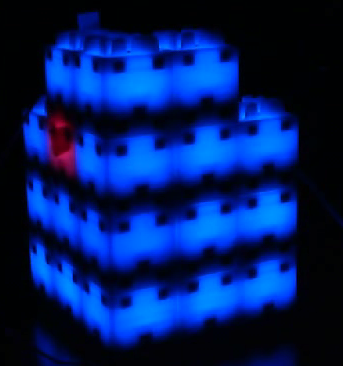
\includegraphics[width=0.75\linewidth]{fig/synchronization/dense}
				\label{fig:system}
			\end{figure}
		\end{column}
		\begin{column}{.53\textwidth}
			\begin{figure}
				\centering
				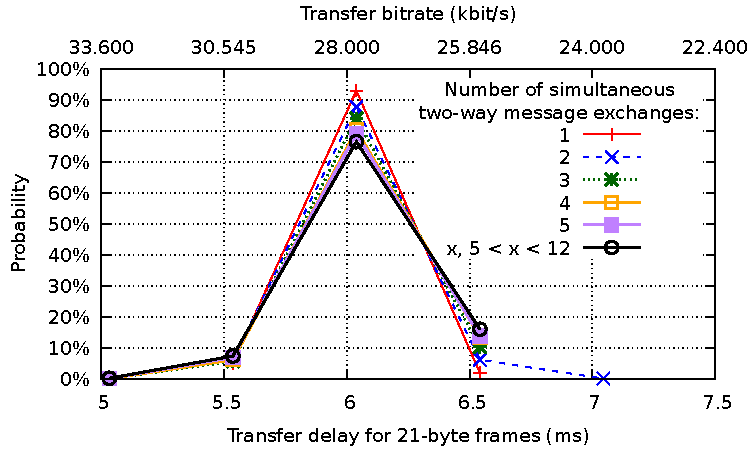
\includegraphics[width=\linewidth]{fig/synchronization/delayNeighborhood}
				\label{fig:transfer-measures}
			\end{figure}
		\end{column}
		\begin{column}{.25\textwidth}	
			300,000 two-way exchanges\\
				~\\$\overline{T_{transfer}} \approx$\\
				 \hspace{1cm} $\frac{\text{frame size}}{28.00}$
		\end{column}
	\end{columns}
	
	\remark{Predictable transfer delays}
\end{center}
\end{frame}

\noLogo{
	\begin{frame} \frametitle{Best Method to Compensate for the Blinky Blocks Communication Delays?}
	
	Methods applicable on the Blinky Blocks
	\begin{itemize}
		\item Predictive (PRED)
		\item Round-Trip Time (RTT): used in TPSN  
		\item Frame Delimiter (FD): used in ATS and MTS
	\end{itemize}
	
	\begin{center}
		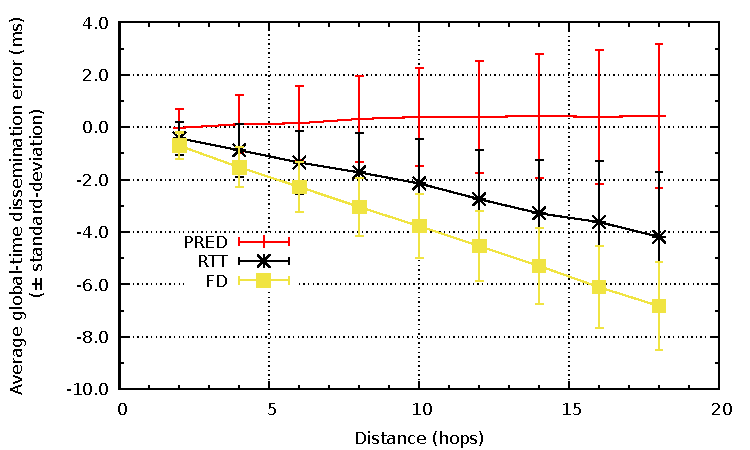
\includegraphics[width=0.6\linewidth]{fig/synchronization/dissemination-error-hw}
		\remark{PRED is the most accurate and uses a single message per hop}
	\end{center}
	\end{frame}
}

\noLogo{
\subsubsection{Hardware Results}

\begin{frame} \frametitle{Synchronizable Radius}
  \centering
  \begin{center}
    \begin{columns}[c]
      \begin{column}{.45\textwidth}
        \centering
        \adjincludegraphics[width=.95\linewidth,valign=t]{fig/synchronization/line1.png}\\
      \end{column}
      \begin{column}{.45\textwidth}
        \centering
        \adjincludegraphics[width=.95\linewidth,valign=t]{fig/synchronization/line2.png}\\
      \end{column}
  \end{columns}
  \end{center}	
  	
  \remark{The time master synchronizes modules in a 27-hop radius to $< 40 ms$}
  \vspace{-1em}
  \begin{center}
  	\begin{columns}[c]
  		\begin{column}{.8\textwidth}
  		\centering
		\remark{Extrapolation: with a central time master, MRTP can synchronize the 27-hop-radius ball system (octahedral shape with 27,775 modules) to $< 40 ms$.}
		\remark{We will use simulations to show it!}
  		\end{column}
  		\begin{column}{.2\textwidth}
  		\centering
  		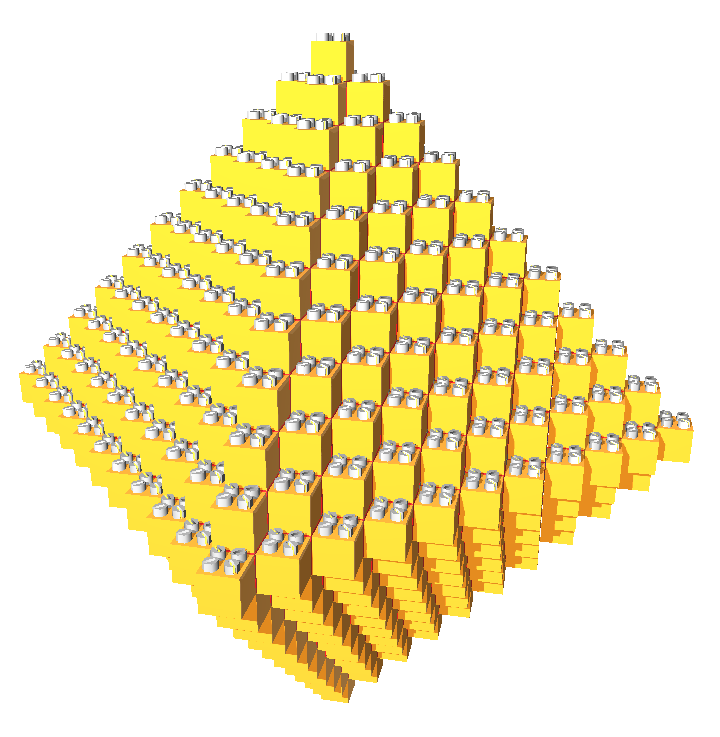
\includegraphics[width=\linewidth]{fig/synchronization/bb-ball-10.png}
  		{\tiny~\\10-hop-radius ball\\\vspace{-1em}1561 Blinky Blocks}
  		\end{column}
  	\end{columns}
  \end{center}
  
\end{frame}
}

\begin{frame} \frametitle{Impact of the Synchronization Period}
  \begin{center}
    \begin{columns}[c]
      \begin{column}{.325\textwidth}
        \centering
        \adjincludegraphics[width=\linewidth,valign=t]{fig/synchronization/L-green.png}\\
        {
        \small
        Duration: 1 hour\\
        Window size: 5
      	}
      \end{column}
      \begin{column}{.675\textwidth}
        \centering
        \adjincludegraphics[width=\linewidth,valign=t]{fig/synchronization/period-hw.pdf}
      \end{column}
  \end{columns}
  \end{center}
  \vfill
  \begin{center}
    \remark{MRTP keeps the system synchronized to a few milliseconds even with a synchronization period of 60 seconds}
    \remark{The synchronization period depends on the desired precision. A long period uses less system resources.}
  \end{center}
\end{frame}

\subsubsection{Simulation Fidelity}

\noLogo{
\begin{frame} \frametitle{VisibleSim Simulator Fidelity}

\begin{center}
	\begin{columns}[c]
		\begin{column}{.35\textwidth}
		Statistical models:
		\begin{itemize}
			\item Clock
				\begin{itemize}
					\item Skew
					\item Drift
					\item Noise (replayed)
				\end{itemize}
			\item Communication time
			\item Processing time
		\end{itemize}
	
		\begin{center}
		\remark{Accurate simulation}
		\end{center}
	
		\end{column}
		\begin{column}{.65\textwidth}
			\footnotesize
			\centering
			Global time dissemination error
			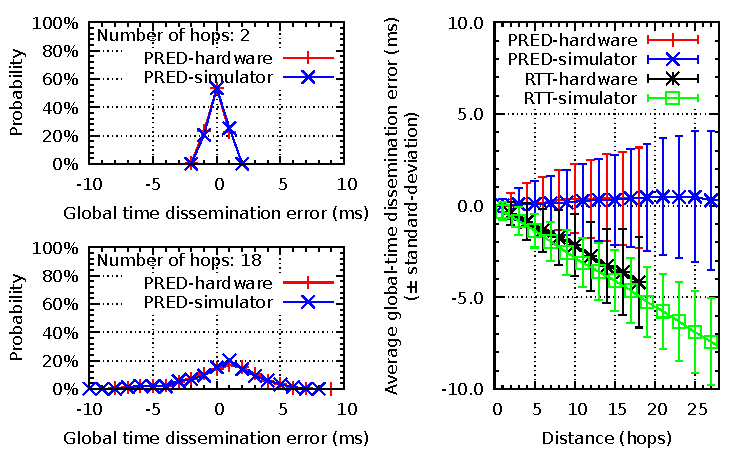
\includegraphics[width=0.75\linewidth]{fig/synchronization/dissemination-error-sim}\\
			Synchronization precision
			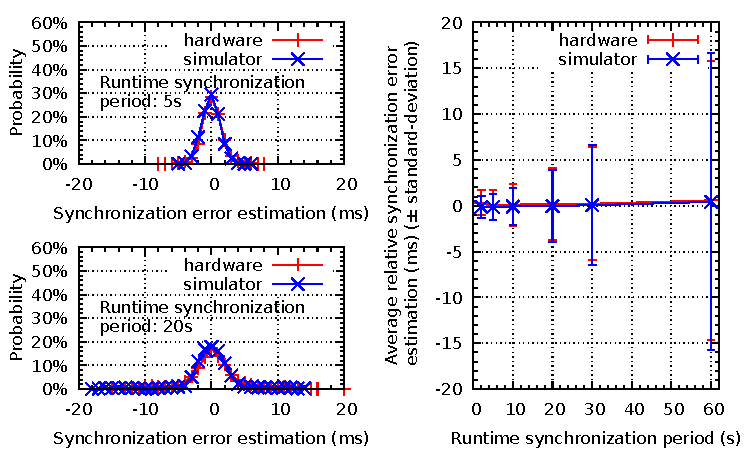
\includegraphics[width=0.75\linewidth]{fig/synchronization/period}
		\end{column}
	\end{columns}
\end{center}
\end{frame}
}

\subsubsection{Simulation Results}

\begin{frame} \frametitle{Simulation Evaluation}

\begin{itemize}
	\item Simulations using VisibleSim
	\item Comparisons with ported version of existing protocols
	\begin{itemize}
		%~\cite{schenato2011average}
		\item Decentralized: ATS [Schenato et al., 2011], WMTS \cite{he2014study} 
		\item Master/Slave with tree: TPSN + MLE \cite{leng2010clock}
		\item Master/Slave but infrastructureless: PulseSync \cite{lenzen2015pulsesync}
	\end{itemize}
	\item Experiments:
	\begin{itemize}
		\item Ball systems (octahedrally-shaped)
		\begin{itemize}
			\item Size: 231 to 27,775 modules
			\item Diameter: 10 to 54 hops
		\end{itemize}
		\item Scenario:
			\begin{itemize}
				\item Left unsynchronized for 1 hour
				\item Then synchronization every 5 seconds during 1 hour
				\item Measurements the maximum pairwise synchronization error every 3 seconds
			\end{itemize}
	\end{itemize}
	\item Evaluation criteria
	\begin{itemize}
		\item Time of convergence
		\item Synchronization precision
		\item Messages
	\end{itemize}
\end{itemize}
\end{frame}

\begin{frame} \frametitle{Convergence Time}

\begin{center}
	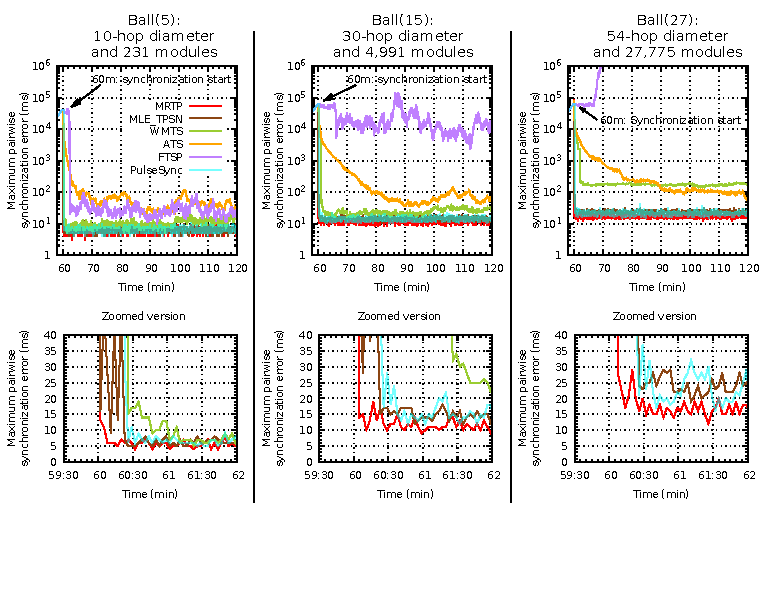
\includegraphics[width=0.9\linewidth]{fig/synchronization/error-time-all-3x2}
\end{center}

\vspace{-1.5cm}
\remark{MRTP converges quickly}

\end{frame}

\begin{frame} \frametitle{Synchronization Precision after Convergence}

\begin{center}
	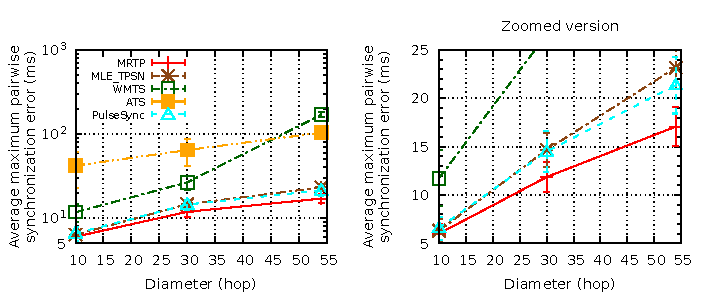
\includegraphics[width=0.9\linewidth]{fig/synchronization/precision}
\end{center}

\remark{MRTP is the most precise protocol}

\remark{MRTP synchronizes the 27,775 module system to 17ms in average}

\end{frame}

\begin{frame} \frametitle{Messages}

\begin{center}
	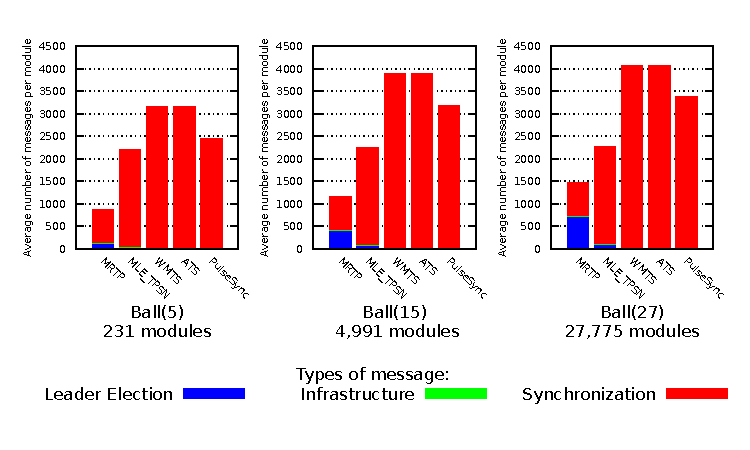
\includegraphics[width=0.9\linewidth]{fig/synchronization/messages}
\end{center}

\remark{MRTP uses few messages}

\end{frame}

\subsection{Conclusion}

\begin{frame} \frametitle{Conclusion}

\begin{itemize}
	\item The Modular Robot Time Protocol (MRTP)
	\item Evaluation
	\begin{itemize}
		\item Hardware
		\item Simulations
		\begin{itemize}
			\item Most precise protocol with a fast convergence
			\item Synchronizes a 27,775 module system with a 54-hop diameter to $< 20ms$ 
			\item Uses less messages in compact systems than existing algorithms
		\end{itemize}
	\end{itemize}
	\item Limit
	\begin{itemize}
		\item Targets fairly stable systems
	\end{itemize}
\end{itemize}
\end{frame}

\section{Self-Reconfiguration}

\subsection{Problem and Motivations}

\begin{frame} \frametitle{Problem and Motivations}

\begin{itemize}
\item Given an initial shape $\mathcal{I}$, a goal shape $\mathcal{G}$ and the mechanical constraints
\item Problem: self-reconfigure the robot from shape $\mathcal{I}$ to $\mathcal{G}$
\begin{center}
	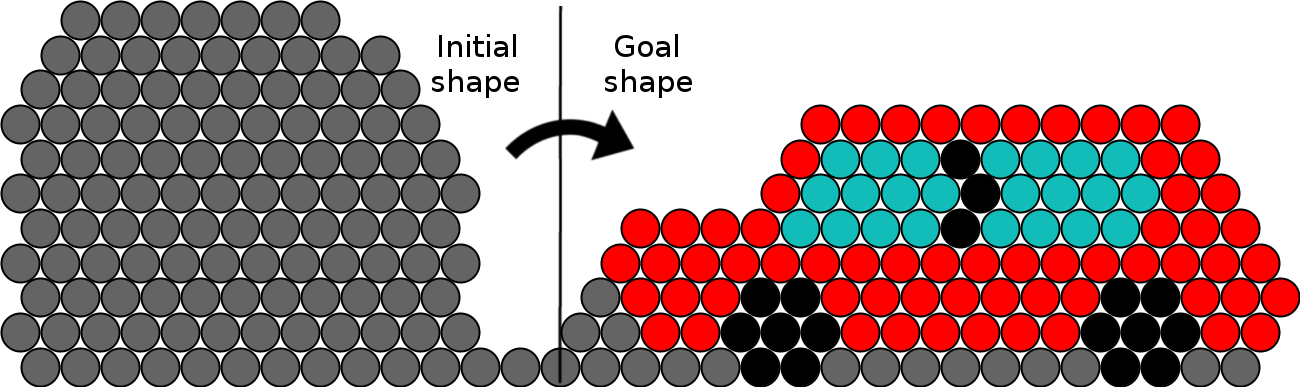
\includegraphics[width=0.6\linewidth]{fig/reconfiguration/car.png}
\end{center}
\item Challenge: Distributed coordination
\begin{itemize}
	\item Effectiveness: reach $\mathcal{G}$
	\begin{itemize}
		\item Prevent collisions
		\item Prevent deadlock %(mechanical constraints) 
	\end{itemize}
	\item Efficiency
	\begin{itemize}
		\item Execution time	
		\item Motion
		\item Communication	
	\end{itemize}
\end{itemize}
\item Motivation: programmable matter
\end{itemize}

\end{frame}

\subsection{System Model and Assumptions}

\noLogo{
\begin{frame} \frametitle{System Model and Assumptions}

\begin{itemize}
\item Hexagonal lattice:
\begin{itemize}
	\item Every module knows its coordinates and its neighbor ones
\end{itemize}
\item Communications:
\begin{itemize}
	\item Asynchronous
	\item Neighbor-to-neighbor only
\end{itemize}
\item Motions:
\begin{itemize}
	\item Asynchronous
	\item Mechanical constraints
	\item No presence sensor: prevent collisions using communications
\end{itemize}
\item Failure-free environment (modules, communications, motions, lattice)
\item Every module stores a complete representation of $\mathcal{G}$
\end{itemize}
\begin{figure}
\vspace{-0.2cm}
\centering
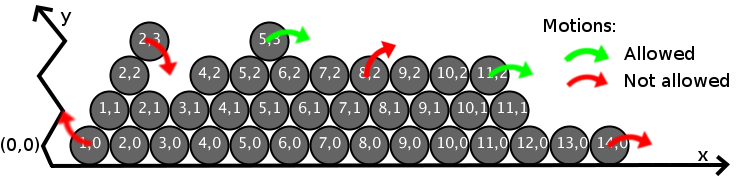
\includegraphics[width=\linewidth]{fig/reconfiguration/model}
\label{fig:model}
\end{figure}
\end{frame}
}


\subsection{Related Work}

{
\newcommand{\lenMinusOne}{0.08\linewidth}
\newcommand{\lenZero}{0.09\linewidth}
\newcommand{\lenOne}{0.12\linewidth}
\newcommand{\lenTwo}{0.14\linewidth}
\newcommand{\lenThree}{0.18\linewidth}
\newcommand{\lenFour}{0.22\linewidth}
\newcommand{\lenFive}{0.27\linewidth}
\newcommand{\lenSix}{0.28\linewidth}

\noLogo{
\begin{frame} \frametitle{Related Work}
{
\scriptsize
\begin{center}
\begin{tabular}{|C{\lenFive}|C{\lenThree}|C{\lenTwo}|C{\lenSix}|}
	\hline
	Cite & Shapes & Constraints on module movement & Collision and deadlock avoidance \\
	\hline
	\cite{walter2000distributed} & \bad{chain to chain} & \bad{relaxed} & centralized pre-computation, synchronous rounds\\
	\hline
	\cite{walter2005algorithms,bateau2012increasing} & \bad{chain to 2D} & \bad{relaxed} & centralized pre-computation, synchronous rounds\\
	\hline
	%lakhlef2015fast
	\cite{lakhlef2015energy} & \bad{chain to square} & \bad{relaxed and very-relaxed} & predefined shape construction\\
	\hline
	\cite{lakhlef2014optimization} & \bad{arbitrary to square} & \bad{relaxed} & predefined shape construction\\
	\hline
	%wong2013deterministic
	\cite{wong2015unpacking} & \bad{compact 2D to chain} & \bad{relaxed} & touch sensors, synchronous rounds, single direction \\
	\hline
	\cite{de2006scalable} & \good{2D} & \bad{relaxed} &  \\
	\hline
	\cite{rubenstein2014programmable} & \good{horizontal 2D compact} & \bad{very relaxed} & collision allowed (swarm robotic) \\
	\hline
\end{tabular}
\end{center}

\begin{center}
\begin{tabular}{|C{\lenFive}|C{\lenThree}|C{\lenTwo}|C{\lenSix}|}
	\hline
	Contribution: C2SR  & \good{vertical 2D compact} & \good{strong} & messages, single direction\\
	\hline
\end{tabular}
\end{center}
}
\end{frame}
}
}


\subsection{Contribution: The Cylindrical-Catoms Self-Reconfiguration (C2SR) Algorithm}

\subsectionOutlineFrame

\subsubsection{Shape Admissibility Conditions}

\noLogo{
\begin{frame} \frametitle{Shape Admissibility Conditions}
% both initial ang goal shapes at the same time
\begin{itemize}
\item $|\mathcal{I}| \geq |\mathcal{G}|$
\item $\mathcal{I}$ and $\mathcal{G}$ are next to each other and share some bottom cells
\item No hole
\item Wide peripheral path with no narrow passage
\end{itemize}
\begin{figure}
\centering
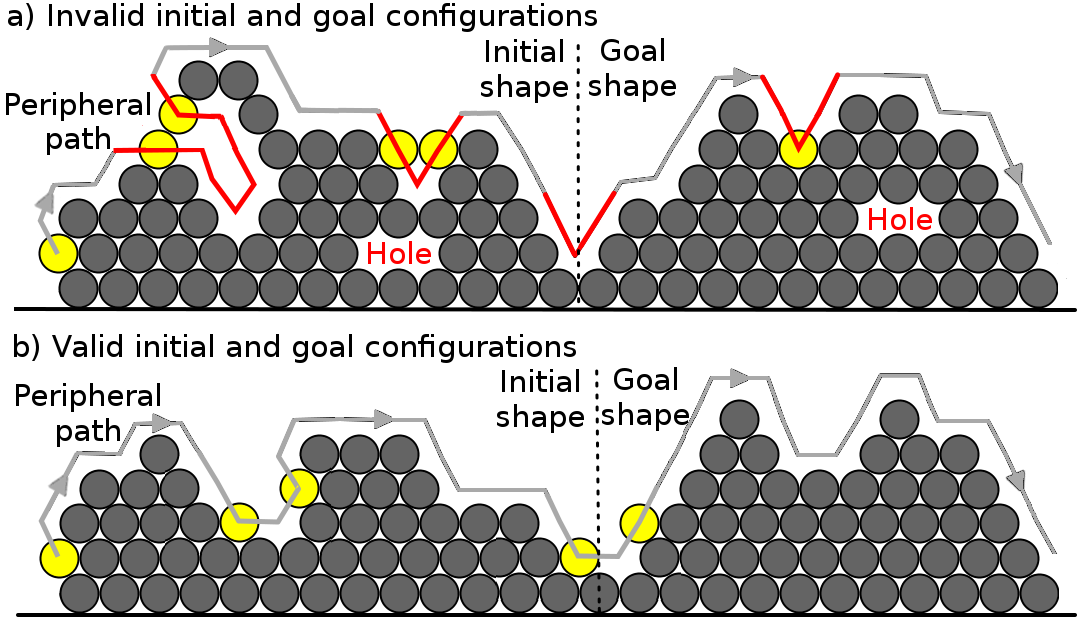
\includegraphics[width=0.75\linewidth]{fig/reconfiguration/admissibility}
\end{figure}
\end{frame}
}

\subsubsection{Algorithm}

\noLogo{
	\begin{frame} \frametitle{C2SR at a Glance}
	\begin{itemize}
	\item Stream of moving modules on the periphery 
	%(CW or CCW)
	\item Maintains an empty cell between moving modules
	\item Layer-by-layer deconstruction/construction (for shapes with only continuous horizontal layers)
	\item Decentralized with local interactions only ($ < 5$ hops)
	\begin{itemize}
		\item Communications with modules geographically around the next position in the stream
	\end{itemize}
	\end{itemize}
	
	\begin{center}
		\begin{columns}[c]
			\begin{column}{.55\textwidth}
				\centering
				\href{run:videos/54-car.avi?autostart&loop}{\adjincludegraphics[width=\linewidth]{videos/54-car.jpg}}
			\end{column}
			\begin{column}{.45\textwidth}
				\centering
				\adjincludegraphics[width=\linewidth,valign=c]{fig/reconfiguration/state-diagram}
			\end{column}
		\end{columns}
	\end{center}	
	\end{frame}
}

\subsection{Evaluation}

\subsubsection{Experimental Setup}

\subsectionOutlineFrame

\noLogo{
\begin{frame} \frametitle{Experiment Setup}

\begin{itemize}
\item VisibleSim
\item Parameters (unless otherwise mentioned)
\begin{itemize}
\item 4 shapes with different scale from $10^1$ to $10^4$ modules
\item Communication rate $\rightarrow \mathcal{N}(38.9 kpbs,389bps)$\ \ \ ($[3ms,8ms]$)
\item Motion speed $\rightarrow \mathcal{N}(1.88 mm \cdot s^{-1},0.0188 mm \cdot s^{-1})$ \ \ \ ($[273ms,285ms]$)
\end{itemize}
\item Evaluation criteria
\begin{itemize}
\item Effectiveness
\item Efficiency
\begin{itemize}
\item Time
\item Motion
\item Communication
\end{itemize}
\end{itemize}
\end{itemize}

%~\\

\begin{columns}[b]
\begin{column}{.24\textwidth}
\centering
\adjincludegraphics[width=\linewidth,height=0.9\linewidth,valign=t]{fig/reconfiguration/car-9644.png}\\
Car
\end{column}
\begin{column}{.24\textwidth}
\centering
\adjincludegraphics[width=\linewidth,height=0.9\linewidth,valign=t]{fig/reconfiguration/flag-12407.png}\\
Flag
\end{column}
\begin{column}{.24\textwidth}
\centering
\adjincludegraphics[width=\linewidth,height=0.9\linewidth,valign=t]{fig/reconfiguration/magnet-10220.png}\\
Magnet
\end{column}
\begin{column}{.24\textwidth}
\centering
\adjincludegraphics[width=\linewidth,height=0.9\linewidth,valign=t]{fig/reconfiguration/pyramid-8033.png}\\
Pyramid
\end{column}
\end{columns}
\end{frame}
}

\subsubsection{Simulation Results}

\definecolor{remarkColor}{RGB}{20,91,155}  % femtost darkblue
\renewcommand{\ResultsScaleFactor}{1}

\newcommand{\NumberExecutionAd}{
\begin{textblock*}{0.5\paperwidth}(0\paperwidth,0.925\paperheight)
\small
*Each point: 10 executions
\end{textblock*}
}

\noLogo{
\begin{frame} \frametitle{Effectiveness: C2SR in Video}

\begin{center}
	
\href{run:videos/57-car1073-x3.avi?autostart&loop}{\includegraphics[width=0.95\linewidth]{videos/57-car1073-x3.jpg}}
\end{center}
\vspace{-0.25cm}
*Speed: x3
\end{frame}
}

\newcommand{\localOutline}[3]{}

\begin{frame} \frametitle{Execution Time ($\pm$ standard-deviation)}

\centering
\begin{tikzpicture}[remember picture,overlay,baseline=-2mm]
\node (image) at (0,-1cm) {\includegraphics[width=\ResultsScaleFactor\linewidth]{./fig/reconfiguration/time}};
\draw[line width=1pt,remarkColor,<-] (2,-1) -- (2.5,-1.50)  node[label={[fill=white,align=center]Linear in the \# modules,\\highly predictable\\ $\frac{1}{0.017} \approx  1$ goal cell/second.}, yshift=-1.825cm, xshift=0.25cm] {};

%59$ goal cell/minute
\end{tikzpicture}
\NumberExecutionAd
\end{frame}

\begin{frame} \frametitle{Average Total Number of Motions ($\pm$ standard-deviation)}
\centering
\begin{tikzpicture}[remember picture,overlay,baseline=-2mm]
\node (image) at (0,-1cm) {\includegraphics[width=\ResultsScaleFactor\linewidth]{fig/reconfiguration/motion}};
\draw[line width=1pt,remarkColor,<-] (1,-1) -- (1.5,-1.50)  node[label={[align=center]Polynomial in the \# modules\\Highly predictable}, yshift=-1.25cm, xshift=0.5cm] {};
\end{tikzpicture}
\NumberExecutionAd
\end{frame}

\begin{frame} \frametitle{Average Number of Messages per Catom ($\pm$ min/max)}

\centering
\begin{tikzpicture}[remember picture,overlay,baseline=-2mm]

\node (image) at (0,-1cm) {\includegraphics[width=\ResultsScaleFactor\linewidth]{fig/reconfiguration/message-individual}};

\draw[line width=1pt,remarkColor,<-] (0.5,-1.5) -- (1,-2.0)  node[label={[align=center]Polynomial in the \# modules\\Highly predictable}, yshift=-1.25cm, xshift=0.5cm] {};

\draw<2>[line width=1pt,remarkColor,->] (1,1.5) -- (0.5,0.5){};
\draw<2>[line width=1pt,remarkColor,->] (1,1.5) -- (-0.75,-0.25){};
\draw<2>[line width=1pt,remarkColor,->] (0.7,1.6) -- (1.7,0.9){};
\draw<2>[line width=1pt,remarkColor] (1.5,1) node[label={[fill=white,align=center]A few modules (at most)\\send a lot more messages}, yshift=0.25cm, xshift=0cm] {};

\node<3> (image) at (0,-1cm) {\includegraphics[width=\ResultsScaleFactor\linewidth]{fig/reconfiguration/parallelism}};
\draw<3>[draw, line width=2pt,remarkColor,label={[xshift=1.0cm, yshift=-0.15cm,align=center]\textcolor{remarkColor}{Communication hotspot}}] (-0.25,-2.5) ellipse (1 and 1);
\node<3>[fill=white] at ($(-0.25,-2)+(75:2 and 1)$) {\textcolor{remarkColor}{Communication hotspot}};
\end{tikzpicture}
\NumberExecutionAd
\end{frame}


\subsection{Conclusion}

\begin{frame}
\frametitle{Conclusion}
\begin{itemize}
	\item The Cylindrical-Catoms Self-Reconfiguration (C2SR) Algorithm
	\begin{itemize}
		\item Effective: tested on different types of shapes
		\item Scalable: tests with more than 10,000 modules
		\item Nice properties:
		\begin{itemize}
		%	\item Local and controlled communications
			\item Execution time seems linear in the size of the goal shape
			\item Highly predictable: number of motions and messages
		\end{itemize}
	\end{itemize}
	\item Limits
	\begin{itemize}
		\item Correctness and performance only shown experimentally
		\item 2D systems only
	\end{itemize}
\end{itemize}
\end{frame}

\section{Conclusion and Future Works}

\begin{frame} \frametitle{Conclusion and Future Works (1)}
\vspace{0.5cm}
\begin{itemize}    
	\item Contributions
	\begin{itemize}
		\item Three efficient algorithms for distributed centrality-based leader election
		\item The Modular Robot Time Protocol (MRTP)
		\item The 2D-Catoms Self-Reconfiguration (C2SR) algorithm
	\end{itemize}
	\vspace{0.5cm}
	\item Future works
	\begin{itemize}
		\item Centrality
		\begin{itemize}
			\item Proofs on the accuracy of our algorithms
			\item Deployment on other platforms with different network structures
			\item More efficient management of network dynamics
		\end{itemize}
		\item Time synchronization
		\begin{itemize}
			\item Deployment on ensembles with more precise clocks
			\item Consider both clock stability and centrality to select the time master
			\item Time synchronization in more dynamic ensembles
			\begin{description}[abc]  % for indentation of length of abc
				\item[$\bullet$] Synchronized self-reconfiguration?
				\item[$\bullet$] For now, PulseSync~\cite{lenzen2015pulsesync} can be used
			\end{description}
		\end{itemize}
	\end{itemize}
\end{itemize}
\end{frame}

% Probalement applicable a dautres platformes pas que robotique modulaire
% pas que: Blinky Blocks
% d'autres primitives
% diffusion des codes sur github

\begin{frame}
\frametitle{Conclusion and Future Works (2)}

\begin{itemize}
	\item Future works (cont'd)
	\begin{itemize}
		\item Self-reconfiguration
		\begin{itemize}
			\item Proof of correctness
			\item Demonstration of the execution time linearity
			\item Other models
			\begin{description}[abc]  % for indentation of length of abc
				\item[$\bullet$] Other mechanical constraints
				\item[$\bullet$] 3D systems
			\end{description} 
		\end{itemize}
	\end{itemize}
\end{itemize}
\end{frame}

\begin{frame} \frametitle{Questions}
  
  \bibliographystyle{apalike}
  \nobibliography{thesis}
  \vspace*{-0.5cm}
  \begin{center}
  	Thank you for your attention!\\
  	~\\
    %Follow us on Google:  {\color{femtostdarkblue}OMNI Team (FEMTO-ST/DISC/OMNI)}\\
    %Visit our project websites:\\
    %Claytronics: {\color{femtostdarkblue}\url{http://www.cs.cmu.edu/~./claytronics/}}\\
    %VisibleSim: {\color{femtostdarkblue}\url{http://projects.femto-st.fr/projet-visiblesim/}}\\
    \includegraphics[keepaspectratio=true,width=.25\paperwidth]{\fileFolder /fig/question-2.png}\\
	Any question?\\
    %{\small Work funded by the Labex Action and ANR}
    ~\\
  {\footnotesize This work has been funded by the ANR/RGC\\(contracts ANR-12-IS02-0004-01 and 3-ZG1F)}
  \end{center}
\end{frame}

%\begin{frame}[noframenumbering] \frametitle{Acknowledgments / Remerciements}
%
%Merci à / Thank you to:
%\begin{itemize}
%	\item Jury members
%	\item Supervisors
%	\item Colleagues (professors, university staff, PhD students)
%	\item Family members
%	\item Friends
%\end{itemize}
%
%\end{frame}

\end{document}
